%-------------------------------------------------------------------------------------------------------------------------------------------
%	PACKAGES AND OTHER DOCUMENT CONFIGURATIONS
%-------------------------------------------------------------------------------------------------------------------------------------------

\documentclass[a4paper,11pt]{article} % Font and paper size

%----------------------------------------------------------------------------------------
%	PACKAGES AND OTHER DOCUMENT CONFIGURATIONS
%----------------------------------------------------------------------------------------

\usepackage[utf8]{inputenc} % Required for inputting international characters
\usepackage[T1]{fontenc} % Output font encoding for international characters
\usepackage[italian]{babel} % Italian dictionary


\usepackage[table]{xcolor} % Required for custom colors
\usepackage{gensymb}
\usepackage{amsmath}
\usepackage{bm}
\usepackage{tikz}
\usepackage{hhline}
\usepackage{listings}
\usepackage{enumitem}

%\usepackage[margin=2cm, includefoot]{geometry} % Modify margins
\usepackage{fancyhdr}
\usepackage{rotating}
\usepackage[hidelinks]{hyperref} % Hyperlinks

\usepackage[none]{hyphenat}% Non spezza le parole nelle tabelle
\usepackage{array}

\usepackage{graphicx} % Required for figures
\usepackage{float}
\usepackage{wrapfig}
\usepackage{caption}
\usepackage{subcaption}

%pagestyle
\pagestyle{fancy}
\fancyhead{}
\fancyfoot{}
\fancyfoot[R]{\thepage}
\renewcommand{\headrulewidth}{0pt}



\usepackage{xfrac}
\usepackage{amssymb}

\usepackage{multicol}
\usepackage{multirow}

\usepackage[toc, page]{appendix}
\usepackage{booktabs}
\usepackage{siunitx}


%----------------------------------------------------------------------------------------
%	NEW COMMANDS
%----------------------------------------------------------------------------------------

\newcommand{\restr}[2]{{% we make the whole thing an ordinary symbol
\left.\kern-\nulldelimiterspace % automatically resize the bar with \right
#1 % the function

\right|_{#2} % this is the delimiter
}}

\newcommand{\tnhl}{\tabularnewline\hline}
\newcommand{\tn}{\tabularnewline}
\newcolumntype{x}[1]{%
	>{\centering\hspace{0pt}}p{#1}}%


 % Include the file specifying document layout and packages


%-------------------------------------------------------------------------------------------------------------------------------------------
%	GENERAL INFORMATION 
%-------------------------------------------------------------------------------------------------------------------------------------------

\newcommand{\labcourse}{Laboratorio di Fisica}
\newcommand{\teacher}{Docenti: Prof. A. Garfagnini - Prof. M. Lunardon}
\newcommand{\laurea}{Corso di Laurea in Fisica}
\newcommand{\channel}{Canale 1 A-L}
\newcommand{\academicyear}{Anno Accademico 2020/2021}
\newcommand{\labexp}{Esperienza di Laboratorio}
\newcommand{\exptitle}{Amplificatori Operazionali \& Calibrazione Arduino}
\newcommand{\turno}{Turno T2}
\newcommand{\name}{Nicolò Lai}
\newcommand{\matricola}{1193976}
\newcommand{\mail}{nicolo.lai@studenti.unipd.it}
\newcommand{\consegna}{Data Esperienza}
\newcommand{\data}{28/10/2020 - 29/10/2020}


%-------------------------------------------------------------------------------------------------------------------------------------------
%	DOCUMENT 
%-------------------------------------------------------------------------------------------------------------------------------------------

\begin{document}

%-------------------------------------------------------------------------------------------------------------------------------------------
%	REFERNCE CUSTOMIZATION
%-------------------------------------------------------------------------------------------------------------------------------------------

\def\sectionautorefname{Sezione} 
\def\subsectionautorefname{Sezione} 
\def\subsubsectionautorefname{Sezione}

%-------------------------------------------------------------------------------------------------------------------------------------------
%	TITLE PAGE
%-------------------------------------------------------------------------------------------------------------------------------------------

\begin{titlepage}
	\begin{center}
		\Huge{\bfseries \labcourse}\\
			
		\LARGE \teacher \\
		\Large \laurea\\
		\Large \channel\\
		\Large \academicyear\\
		[1cm] 
		\line(1,0){400}\\
		[3.5cm]
			
		\textsc{\huge{\bfseries \labexp}}\\
		\huge{\exptitle}\\
		[2mm] \line(1,0){300}\\
		[10cm]
	\end{center}
	
	
	\begin{flushleft}
		\textsc{\Large \turno}\\
		[0.5cm] \textsc{\large {\bfseries \name}} \\ 
		\indent\large \matricola \\ 
		\indent\large \mail \\
	\end{flushleft}
		
					
	\begin{flushright}
			\textsc{\Large\consegna}\\
			\textsc{\large \data}					
	\end{flushright}
			
\end{titlepage}
\cleardoublepage


%-------------------------------------------------------------------------------------------------------------------------------------------
%	OBIETTIVO
%-------------------------------------------------------------------------------------------------------------------------------------------

\section{Obiettivo}

Verificare la linearità di un amplificatore operazionale e misurare il guadagno di un circuito che lo comprenda.
Misurare la frequenza di taglio di un filtro attivo. Calcolare il sampling rate e la funzione di calibrazione in
tensione di una scheda Arduino Due.

%-------------------------------------------------------------------------------------------------------------------------------------------
%	APPARATO SPERIMENTALE
%-------------------------------------------------------------------------------------------------------------------------------------------

\section{Strumentazione e Componenti}\label{s:strumenti}

Nel corso dell'esperienza vengono utilizzati:
\begin{itemize}
	\item Multimetro digitale Metrix MTX3292
	\item Generatore di funzioni Tektronix AFG1022
	\item Oscilloscopio digitale Tektronix TBS1102B
	\item Alimentatore di tensione continua TTi
	\item Circuito integrato TL082C (contenente due amplificatori operazionali)
	\item Tre resistori $R_{\text{f}}$, $R_{1}$, $R_{3}$ ed un condensatore $C_{1}$ 
	\item Scheda Arduino Due
\end{itemize}


%-------------------------------------------------------------------------------------------------------------------------------------------
%	AMPLIFICATORE OPERAZIONALE INVERTENTE
%-------------------------------------------------------------------------------------------------------------------------------------------

\section{Amplificatore Operazionale Invertente}\label{s:opamp} 

In questa sezione ci si propone di studiare il comportamento di un circuito puramente resistivo comprendente un
amplificatore operazionale in configurazione invertente (polo positivo a massa, polo negativo collegato al segnale in
ingresso). Si vuole in particolare verificare la sua linearità e stimare l'amplificazione del circuito come grandezza
derivata sia partendo dalle misure dirette delle resistenze del circuito, sia come parametro di un'interpolazione
lineare di misure acquisite con l'oscilloscopio. 


%-------------------------------------------------------------------------------------------------------------------------------------------
%	CONFIGURAZIONE SPERIMENTALE
%-------------------------------------------------------------------------------------------------------------------------------------------

\subsection{Configurazione Sperimentale}\label{s:guadagno}

Si inizia assemblando il circuito, rappresentato in \autoref{i:opamp_circuit}, utilizzando le resistenze $R_{\text{f}}$, $R_1$,
$R_3$ e l'amplificatore operazionale. La resistenza $R_{\text{g}}$ rappresenta la resistenza interna del generatore, non nulla in
quanto ci si trova in condizioni di non idealità. Le resistenze esterne, invece, vengono misurate

\begin{wrapfigure}{R}{0.6\textwidth}
	\centering
	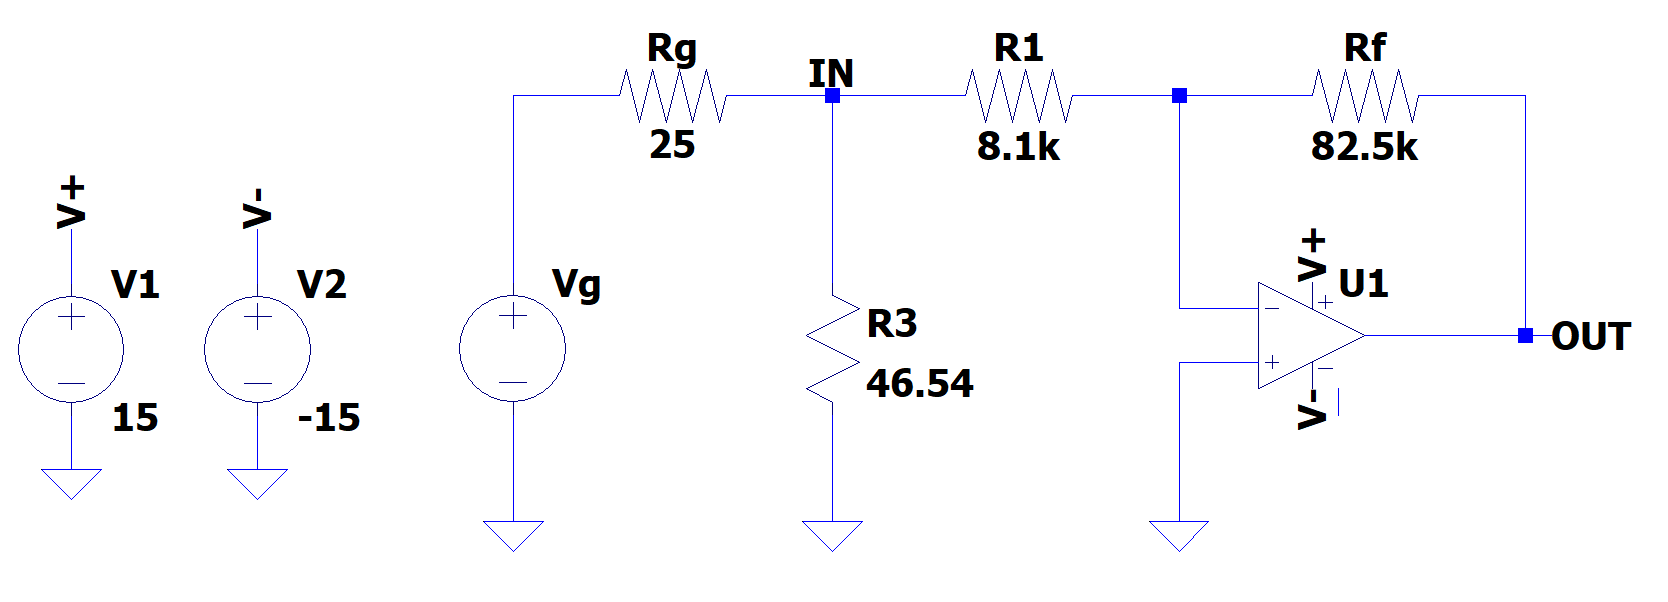
\includegraphics[width=0.6\textwidth]{../Simulations/OpAmp/circuit_image_nosim.png}
	\caption{\footnotesize Rappresentazione a variabili concentrate del circuito assemblato in laboratorio.}
	\label{i:opamp_circuit}
\end{wrapfigure}

\noindent direttamente utilizzando il multimetro Metrix MTX3292, ottenendo i risultati esposti in
\autoref{t:direct_measures}. Si utilizza poi un generatore di tensione continua con $V_{\text{cc}}=+15\,\si{\volt}$ e
$V_{\text{ee}}=-15\,\si{\volt}$ per l'alimentazione dell'amplificatore operazionale. Si assume, inoltre, che esso abbia
un comportamento ideale, ovvero che il polo positivo ed il polo negativo si trovino allo stesso potenziale. Il segnale
viene prelevato nei punti \textit{IN} e \textit{OUT} evidenziati nello schema in \autoref{i:opamp_circuit} (e verrà in
seguito richiamato rispettivamente come $V_{\text{in}}$ e $V_{\text{out}}$) utilizzando due sonde con fattore di
attenuazione 10X. Nel canale CH1 dell'oscilloscopio viene visualizzato il segnale in ingresso $V_{\text{in}}$, mentre il
segnale in uscita $V_{\text{out}}$ è prelevato dalla sonda collegata al canale CH2. Per entrambi i canali viene
selezionata la modalità "attenuazione sonda 10X", in modo da compensare la riduzione del segnale dovuta alle sonde e
visualizzare quindi nel display il segnale reale. Il generatore di funzioni viene poi configurato in

\begin{wraptable}{L}{0.5\textwidth}
	\small
	\centering
	\begin{tabular}{x{1.8cm} x{2.5cm} x{2cm} } \toprule[0.5px]\toprule[0.1px]
		
		\multicolumn{3}{c}{Misure Dirette delle Resistenze}\tn
		\midrule[0.1px]
		
		Resistenza & Valore & F.S. \tn
		
		\addlinespace
		
		$R_{\text{f}}$ & $82.46 \pm 0.03\,\si{k\ohm}$ & $100\,\si{k\ohm}$ \tn

		$R_1$ & $8.089 \pm 0.003\,\si{k\ohm}$ & $10\,\si{k\ohm}$ \tn

		$R_3$ & $46.54 \pm 0.05\,\si{\ohm}$ & $1\,\si{k\ohm}$ \tn
		
		\bottomrule[0.5px]		
	\end{tabular}
	\caption{\footnotesize Valori di resistenza, misurati direttamente con il multimetro, e relativo fondoscala.}
	\label{t:direct_measures}
\end{wraptable}	

\noindent  modalità "50 Ohm", in modo che l'impedenza d'uscita del generatore sia comparabile con
$R_3\approx 50\,\si{\ohm}$. Ci si aspetta così di trovare una tensione in ingresso $V_{\text{in}}$ in accordo con la
tensione nominale erogata dal generatore. Si imposta infine il generatore di funzioni in modo da erogare un segnale di
tipo sinusoidale con frequenza $f_{\text{gen}}=1\,\si{k\hertz}$, mantenuta costante in questa sezione, e di ampiezza
invece variabile tra $200\,\si{\mV}$ picco picco e $3.5\,\si{\V}$ picco picco. \\

\noindent Dall'assunzione di idealità dell'amplificatore operazionale segue che, risolvendo il circuito, il segnale in
uscita è legato a quello in ingresso da $V_{\text{out}} = - R_{\text{f}} / R_{1} \, V_{\text{in}}$, dove il segno meno
(dovuto alla particolare configurazione dell'operazionale) indica un segnale in output invertito\footnote{Ci si aspetta
che i massimi del segnale in ingresso corrispondano ai minimi del segnale in uscita e viceversa.} rispetto a quello in
ingresso, e amplificato di un fattore $G \equiv R_{\text{f}} / R_{1}$. Facendo riferimento ai valori
delle resistenze $R_{\text{f}}$ ed $R_1$ riportate in \autoref{t:direct_measures}, l'aspettativa teorica per il guadagno
del circuito è dunque 
\begin{align}\label{e:guadagno}
	G&=\frac{R_{\text{f}}}{R_{1}} = 10.194 \pm 0.006
	&
	\text{con   }\,\,\sigma_{G}&=\sqrt{	\left(	\frac{	1	}{	R_{1}	}	\right)^2	\sigma_{R_{\text{f}}}^2	
	+	\left(	\frac{	R_{\text{f}}	}{	R_{1}^2	}	\right)^2\sigma_{R_{1}}^2	}
\end{align}

%-------------------------------------------------------------------------------------------------------------------------------------------
%	SIMULAZIONE SPICE PRELIMINARE
%-------------------------------------------------------------------------------------------------------------------------------------------

\subsubsection{Simulazione Spice del Circuito}\label{s:spice} 

Si decide di effettuare una simulazione della risposta del circuito ad un segnale sinusoidale di frequenza
$f_{\text{gen}}=1\,\si{k\hertz}$ in ingresso, come da configurazione sperimentale. In \autoref{i:opamp_simulation} sono
rappresentate due 

\begin{wrapfigure}{L}{0.5\textwidth}
	\centering
	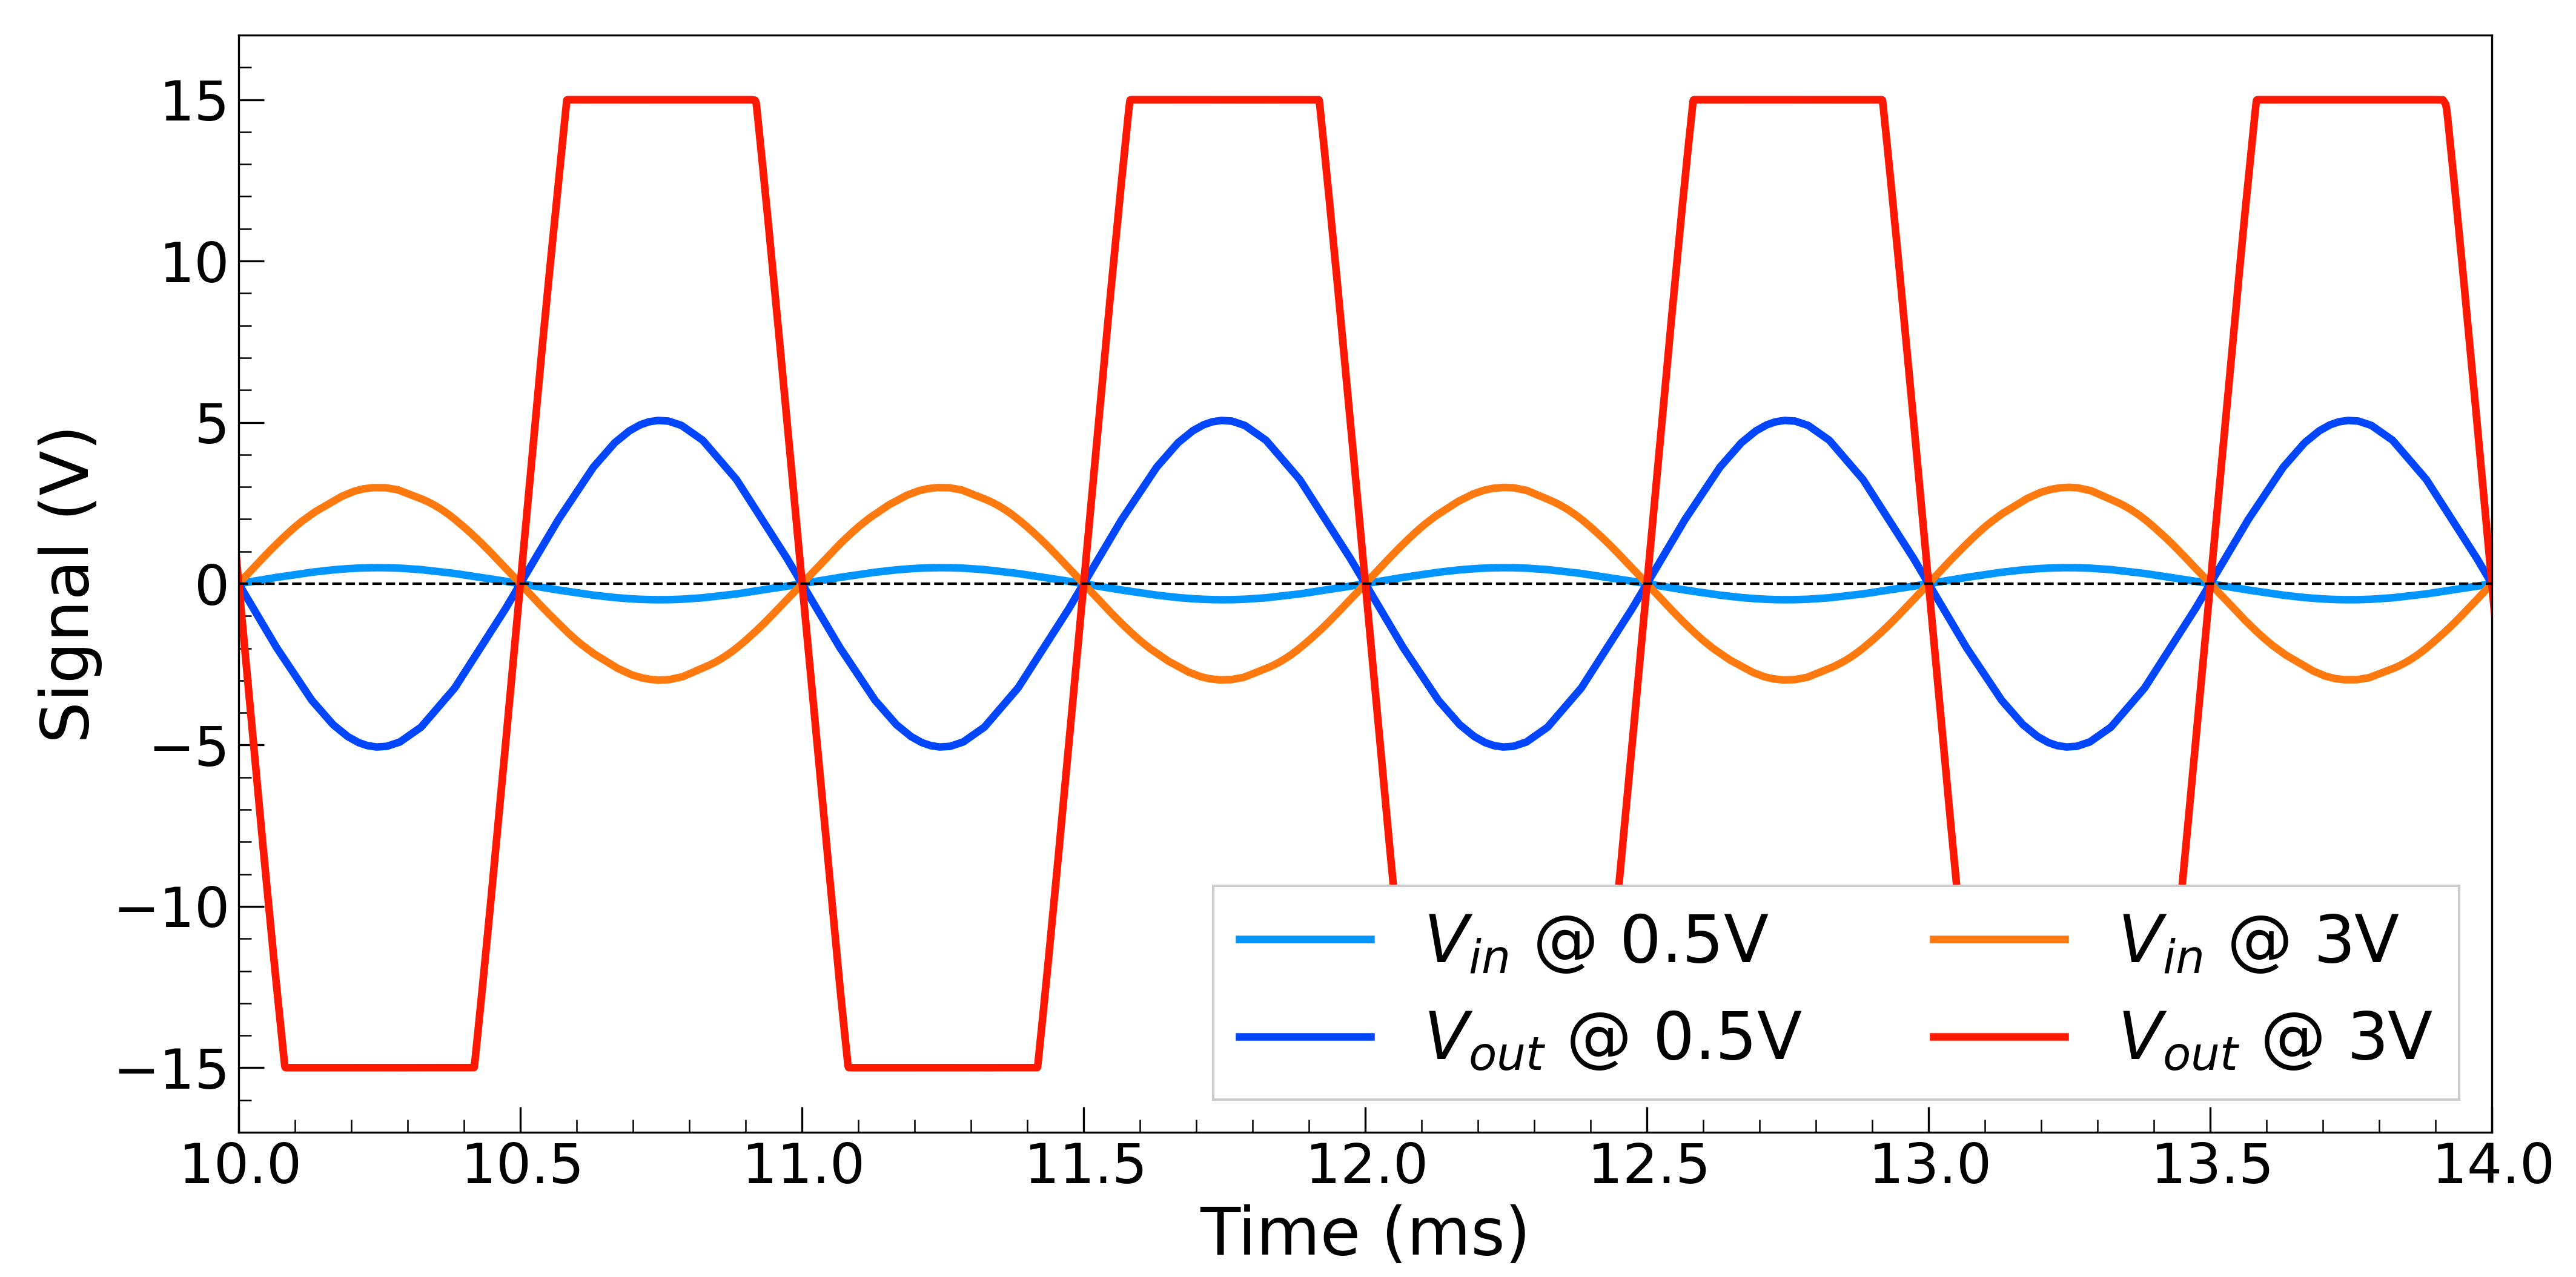
\includegraphics[width=0.5\textwidth]{../Plots/Report_Plots/opamp_spice_py.png}
	\caption{\footnotesize Simulazione Spice della risposta del circuito.}
	\label{i:opamp_simulation}
\end{wrapfigure}

\noindent simulazioni corrispondenti a due ampiezze differenti del segnale in ingresso: la prima (in tonalità
\textit{blu}) è la risposta a $V_{\text{gen}}=0.5\,\si{\volt}$, mentre la seconda (in tonalità \textit{rossa}) a
$V_{\text{gen}}=3\,\si{\volt}$. Dal grafico si nota chiaramente come la risposta $V_{\text{out}}$ ad un segnale in
ingresso $V_{\text{gen}}=0.5\,\si{\volt}$ sia perfettamente conforme alle aspettative: viene mantenuta la forma
sinusoidale del segnale, amplificato di circa un fattore 10 ed invertito rispetto alla tensione $V_{\text{in}}$. Si nota
inoltre come questo non si ripresenti anche nel caso della risposta a $V_{\text{gen}}=3\,\si{\volt}$: il segnale in
uscita presenta, infatti, i picchi di massimo e minimo tagliati a livello $V_{\text{sat}}=\pm 15\,\si{\volt}$. Questo
accade perchè, essendo l'amplificatore operazionale una componente attiva del circuito, è stato alimentato con una
tensione continua a $\pm 15\,\si{\volt}$ (come riportato sopra). Per la conservazione dell'energia, allora, l'operazionale
non può fornire in output una tensione maggiore di quanta ne riceve esso stesso in alimentazione. Si parla quindi di
\textit{saturazione} del segnale in uscita a $V_{\text{sat}}=\pm 15\,\si{\volt}$. Per quanto detto,  avendo $G \approx
10$, ci si aspetta che questo fenomeno inizi a manifestarsi attorno ad un valore nominale di tensione
$V_{\text{gen}}=1.5\,\si{\volt}$.


%-------------------------------------------------------------------------------------------------------------------------------------------
%	ACQUISIZIONE MISURE
%-------------------------------------------------------------------------------------------------------------------------------------------

\subsection{Acquisizione Misure}

Al fine di verificare la linearità dell'amplificatore operazionale e stimare l'amplificazione $G$ del circuito, vengono
acquisite separatamente le misure di un massimo ed un minimo sia del segnale in ingresso sia di quello in uscita facendo
variare la tensione nominale erogata dal generatore partedo da $200\,\si{\mV}$ picco picco fino a $3.5\,\si{\volt}$ picco
picco. Per l'acquisizione vengono utilizzati i cursori di tipo tensione dell'oscilloscopio (orizzontali). 


%-------------------------------------------------------------------------------------------------------------------------------------------
%	DATI E ANALISI
%-------------------------------------------------------------------------------------------------------------------------------------------

\subsection{Dati e Analisi}

In questa sezione si vuole inizialmente rappresentare le misure acquisite in laboratorio riportandole in un grafico
esplorativo di $V_{\text{out}}$ contro $V_{\text{in}}$: da questo si cerca dunque di estrarre informazioni di carattere
generale riguardo i dati a disposizione. Le coppie $\{V_{\text{in}},\,V_{\text{out}}\}$ sono costruite associando, per
ogni valore di tensione nominale erogata dal generatore, il massimo di $V_{\text{out}}$ al rispettivo massimo di
$V_{\text{in}}$ (analogo per i minimi). Per quanto riportato in \autoref{s:guadagno} ci si aspetta una distribuzione
lineare delle coppie con pendenza pari all'amplificazione del circuito $G$: attraverso un'interpolazione lineare,
quindi, è possibile estrarre una stima di tale $G$. Inoltre è possibile caratterizzare la linearità dell'operazionale
tramite la bontà del fit e studiando l'andamento dei residui associati all'interpolazione.


%-------------------------------------------------------------------------------------------------------------------------------------------
%	DATISET
%-------------------------------------------------------------------------------------------------------------------------------------------

\subsubsection{Dataset}

Si comincia riportando in \autoref{i:opamp_eda} le misure acquisite con l'oscilloscopio, alle quali (sia a
$V_{\text{in}}$ sia a $V_{\text{out}}$) si associa la seguente incertezza:
\begin{equation}\label{e:osc}
	\sigma_{V} = \sqrt{ (\sigma_{\text{L}}\times\text{V/div})^2 + (\sigma_{\text{k}}\times\text{measure})^2 }
\end{equation}
\noindent dove $\sigma_{\text{L}}=0.04$ rappresenta il contributo di lettura e $\sigma_{\text{k}}=1.5\%$ il contributo di scala
associati all'oscilloscopio mentre V/div rappresenta la scala di acquisizione della misura.
\begin{figure}[H]
	\centering
	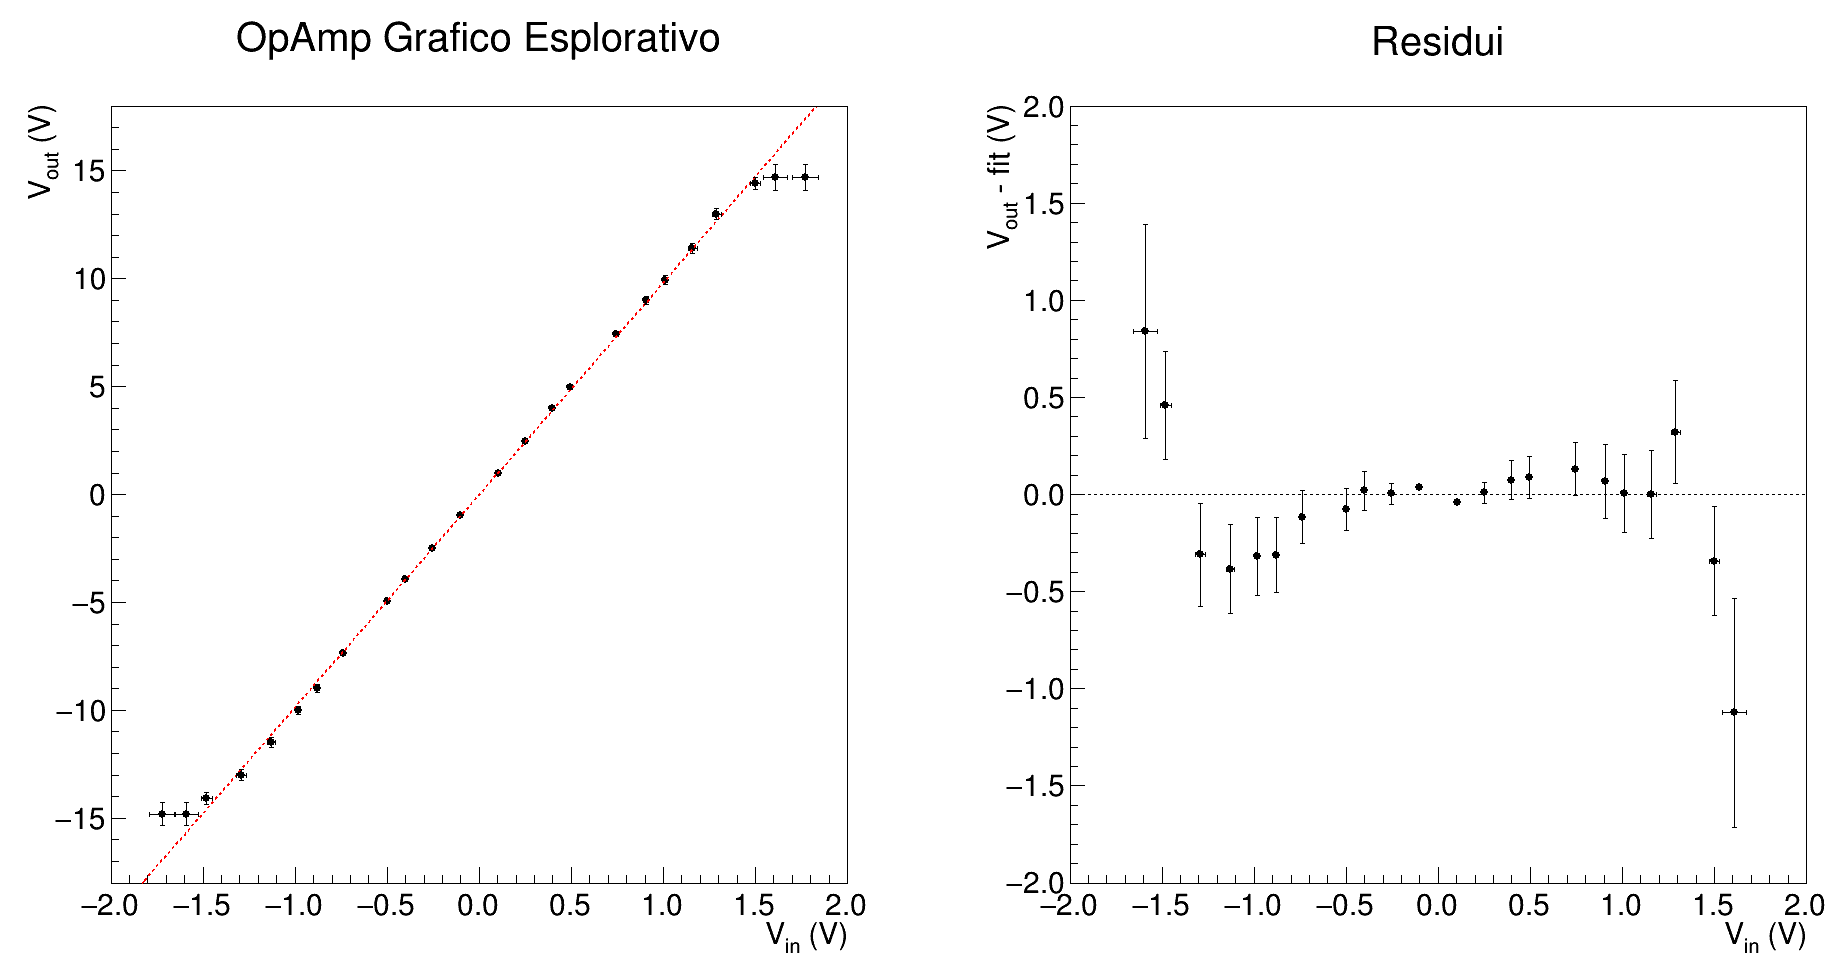
\includegraphics[width=\linewidth]{../Plots/Report_Plots/opamp_plot_alldata_eda.png}
	\caption{\small Grafico delle misure acquisite interpolate linearmente e relativo grafico dei residui.}
	\label{i:opamp_eda}
\end{figure}
\noindent Si noti inizialmente che i valori di $V_{\text{in}}$ sono conformi a quanto erogato dal generatore: questo è
sicuramente indice di una corretta acquisizione del segnale in ingresso, di una corretta configurazione del genetratore
(modalità "50 Ohm") e dell'oscilloscopio (attenuazione sonda 10X). Osservando poi i valori di $V_{\text{out}}$, si nota
un'amplificazione conforme alle aspettative (circa di un fattore 10). Si osserva, inoltre, come le misure acquisite a
$V_{\text{gen}}\approx 1.5\,\si{\volt}$ tendano a stabilizzarsi attorno a $V_{\text{out}}=V_{\text{sat}}=\pm
15\,\si{\volt}$, ovvero la tensione massima che l'amplificatore operazionale può fornire in output: questo effetto di
saturazione del segnale in uscita segue le previsioni esposte in \autoref{s:spice}. Spostando l'attenzione sul grafico
dei residui, si può notare chiaramente che l'effetto della saturazione del segnale si traduce qui in outliers rispetto
al trend lineare dei dati, i quali residui si distribuiscono invece ragionevolmente attorno allo zero. Si noti infine
come gli errori relativi $\sigma_{V_{\text{in}}}/V_{\text{in}}$ e $\sigma_{V_{\text{out}}}/V_{\text{out}}$ siano
generalmente comparabili tra loro: le incertezze su $V_{\text{in}}$ non sono quindi trascurabili rispetto a quelle su
$V_{\text{out}}$.


%-------------------------------------------------------------------------------------------------------------------------------------------
%	PRELIMIARY FIT
%-------------------------------------------------------------------------------------------------------------------------------------------

\subsubsection{Linearità e Amplificazione}\label{s:pre} 

Si procede ora considerando il campione di coppie $\{V_{\text{in}},\,V_{\text{out}}\}_{\text{MAX}}$ corrispondente alle
misure di massimo e $\{V_{\text{in}},\,V_{\text{out}}\}_{\text{MIN}}$ di minimo separatamente. A priori, infatti, non si
ha la certezza che i due siano caratterizzati dalla stessa amplificazione $G$ e che non sia presente una sistematica di
shift/offset verticale tra dataset. Si utilizzeranno quindi le informazioni sui parametri delle rispettive rette
interpolanti per quantificare l'accordo tra i due campioni di misure. Chiaramente, nelle interpolazioni successive, non
verranno considerati gli outliers identificati nella sezione precedente. Si è notato, inoltre, come l'errore sulle
misure di $V_{\text{in}}$ non sia trascurabile rispetto a quello su $V_{\text{out}}$. Per tenere conto di questo, ci si
propone allora di effettuare un fit preliminare nel quale si considera unicamente l'errore su $V_{\text{out}}$. Il
coefficiente angolare $m$ della retta viene dunque utilizzato per proiettare il contributo di incertezza dovuto a
$V_{\text{out}}$ lungo l'asse delle ordinate secondo
\begin{equation}\label{e:proj}
	\sigma_{y} = \sqrt{	\sigma_{V_{\text{out}}}^2	+	m^2	\sigma_{V_{\text{in}}}^2	}
\end{equation}
\noindent I coefficienti angolari di interesse sono dunque riportati in  \autoref{t:pre_slopes}.
\begin{table}[H]
	\small
	\centering
	\begin{tabular}{x{4cm} x{4cm}} 

		\toprule[0.5px]
		\toprule[0.1px]
		
		\multicolumn{2}{c}{Coefficienti Angolari Preliminari}\tn
		\midrule[0.1px]

		Campione di Massimi & Campione di Minimi \tn

		\addlinespace
		
		$m=10.02\pm0.09$ & $m=10.16\pm0.09$ \tn
		
		\bottomrule[0.5px]
		
	\end{tabular}
	\caption{\small Valori dei coefficienti angolari restituiti dalle interpolazioni preliminari.}
	\label{t:pre_slopes}
\end{table}	
%-------------------------------------------------------------------------------------------------------------------------------------------
%	LINEARITA E AMPLIFICAZIONE
%-------------------------------------------------------------------------------------------------------------------------------------------
\noindent Si ripetono ora le interpolazioni dei due dataset con il contributo d'errore proiettato. I parametri restituiti
da tali fit sono riportati in  \autoref{t:opamp_fitres_max_min}.
\begin{table}[H]
	\centering
	\small
	\begin{tabular}{x{3cm} x{3cm} x{3cm} x{3cm}} 

		\toprule[0.5px]
		\toprule[0.1px]
		
		\multicolumn{4}{c}{Fit Parameters}\tn
		\midrule[0.1px]

		\multicolumn{4}{c}{Campione di Massimi}\tn

		\addlinespace
		
		Offset (V) & Slope & $\chi^2$/ndf & $\sigma_{\text{posteriori}}$ (V)\tn

		\addlinespace

		$-0.06\pm0.04$ & $10.02\pm0.14$ & $0.98/7$ & $0.10$ \tn

		\midrule[0.1px]
		
		\multicolumn{4}{c}{Campione di Minimi}\tn

		\addlinespace
		
		Offset (V) & Slope & $\chi^2$/ndf & $\sigma_{\text{posteriori}}$ (V) \tn

		$0.07\pm0.04$ & $10.16\pm0.14$ & $0.67/7$ & $0.07$ \tn



		\bottomrule[0.5px]
		
	\end{tabular}
	\caption{\small Parametri della retta interpolante, il valore del $\chi^2$ associato al fit 
	e l'errore a posteriori relativo alla distribuzione dei dati.}
	\label{t:opamp_fitres_max_min}
\end{table}	
\noindent Si noti inizialmente come i due coefficienti angolari, che si ricorda rappresentano l'amplificazione risentita
dal segnale in uscita rispetto a quello in ingresso, siano in ottima compatibilità tra loro ($\lambda=0.7$). Da questo,
allora, si può assumere che i due campioni risentano della stessa amplificazione $G$ e che questa è conforme a quanto
trovato in \autoref{e:guadagno}, come da aspettative. Le due stime dell'intercetta $q$ sono invece in leggera
compatibilità con zero ($\lambda \approx 1.5$), mentre tra loro presentano una compatibilità $\lambda=2.4$. Sorge dunque
l'idea di una possibile sistematica di shift/offset verticale tra i due dataset: computando la differenza tra le due
intercette si trova uno sfalsamento $d=0.13 \pm 0.05 \,\si{\volt}$. Osservando poi il valore dei $\chi^2$, si trova per
entrambi i campioni $\chi^2/\text{ndf} \ll 1$. Ricordando che le incertezze sul guadagno verticale dell'oscilloscopio
sono almeno parzialmente correlate, gli errori associati alle misure sono dunque tra loro correlati: questo spiega i
valori di $\chi^2$ eccessivamente ridotti. Un'interpolazione di misure con incertezze correlate restituisce di
conseguenza parametri con errori sottostimati, in quanto il fit non tiene conto di tale correlazione. Si vuole dunque
assumere che i parametri \textit{slope} e \textit{offset} riportati in \autoref{t:opamp_fitres_max_min} presentino in
realtà un accordo maggiore tra i due campioni di misure proprio a causa di una possibile sottostima dell'errore sui
parametri, che però non si riesce a quantificare. Si vuole allora assumere che i due campioni risentano della stessa
amplificazione $G$ e che non siano tra loro sfalsati verticalmente in modo significativo: segue quindi un tentativo di
"unificazione" del campione di dati ed un'interpolazione lineare unica che tenga conto sia dei massimi che dei minimi,
rappresentato in \autoref{i:opamp_all_proj}. 
\begin{figure}[H]
	\centering
	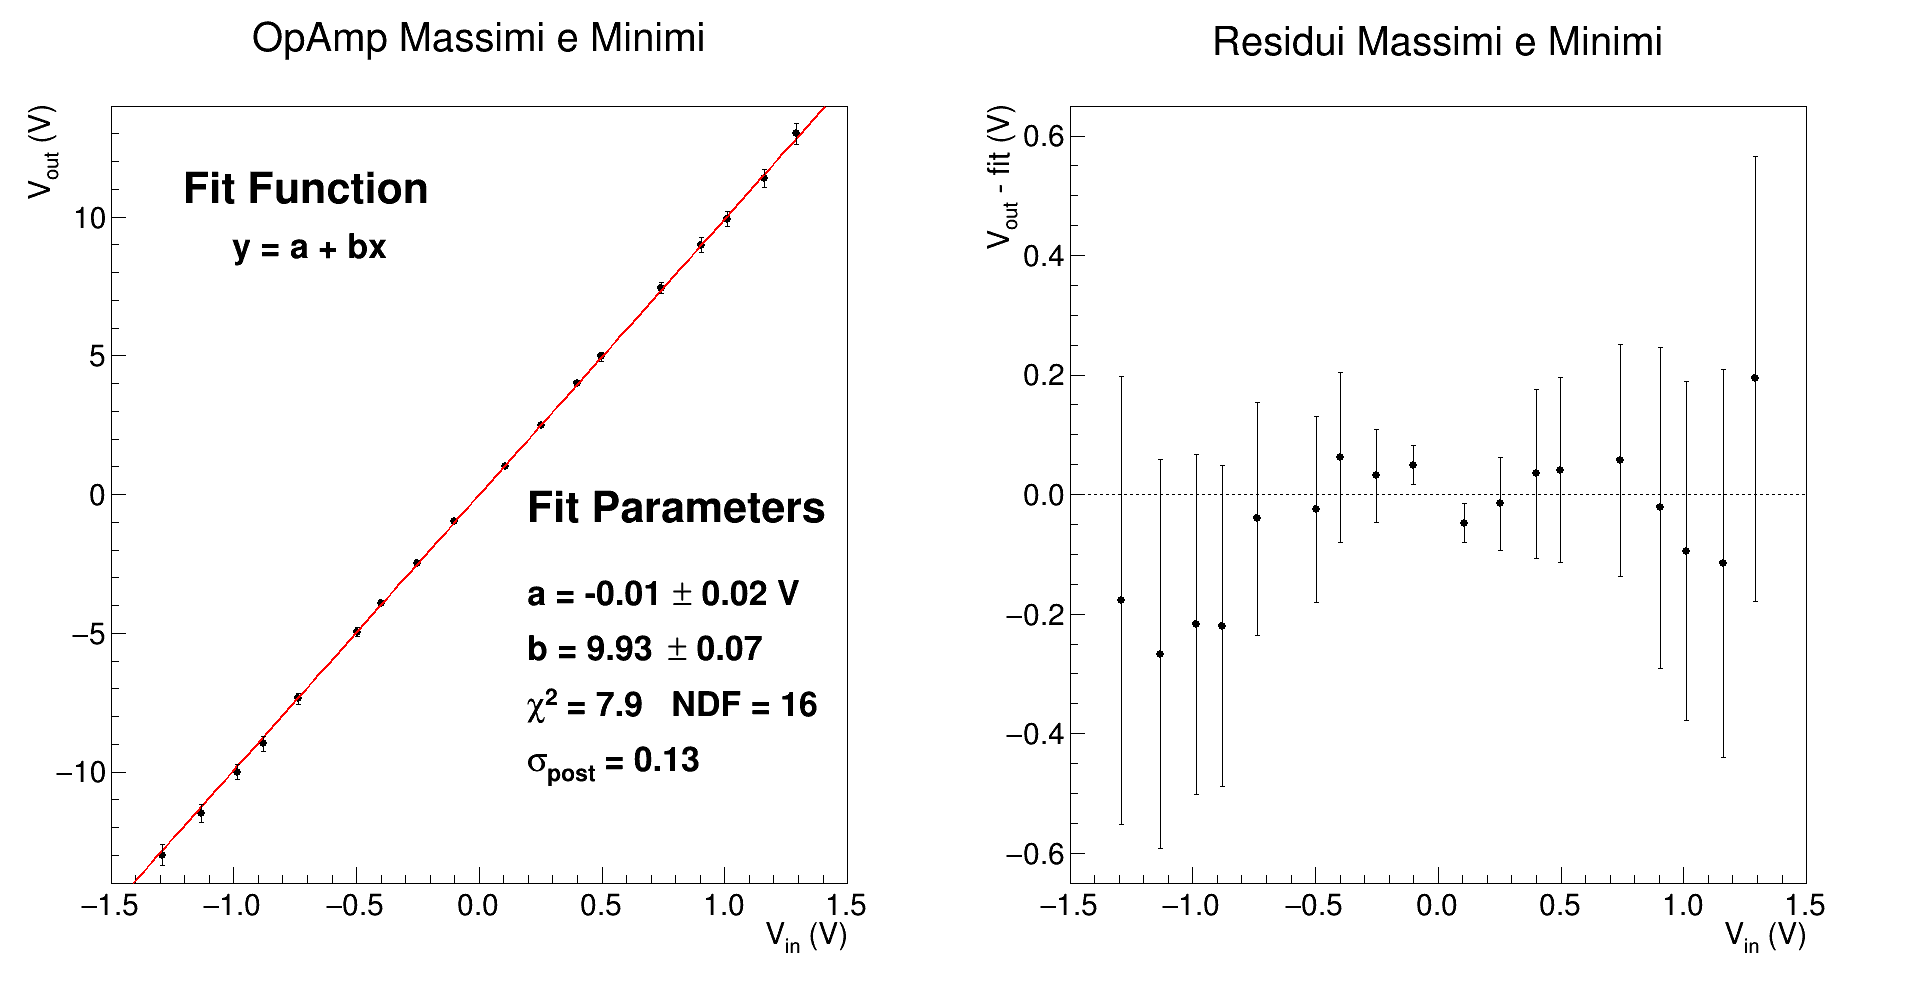
\includegraphics[width=\linewidth]{../Plots/Report_Plots/opamp_plot_all_projected.png}
	\caption{\small A sinistra: grafico rappresentante il dataset dei massimi ed il dataset dei minimi uniti assieme, 
	con relativa retta interpolante e parametri del fit. A destra: grafico dei residui $V_{\text{out}}-\text{fit}$.}
	\label{i:opamp_all_proj}
\end{figure}
\noindent Si noti inizialmente come l'intercetta $a$ risulti ora ben compatibile con zero. Il coefficiente angolare $b$,
invece, pur essendo compatibile con i risultati esposti precedentemente in \autoref{t:opamp_fitres_max_min}, si trova
essere sensibilmente minore di entrambi. Questa "anomalia" è perfettamente conforme con lo sfalsamento $d$ tra i due
campioni: avendo il dataset di minimi un offset positivo e quello dei massimi un offset negativo, il primo si trova
essere "rialzato" rispetto al secondo e la retta interpolante il campione unificato presenta quindi un coefficiente
angolare minore rispetto ai due coefficienti angolari separati. Osservando poi il grafico dei residui, si può notare un
andamento leggermente patologico, quasi parabolico, avente concavità rivolta verso il basso: è evidente come questo
andamento sia dovuto alla sistematica di sfalsamento tra i due dataset. Si può inoltre notare un andamento "a farfalla"
delle barre d'errore, tipico della correlazione degli errori tra misure acquisite con l'oscilloscopio. L'errore a
posteriori, tuttavia, si trova in una zona intermedia rispetto alla gamma di errori associati alle misure: non potendo
eliminare la correlazione tra le incertezze si può affermare dunque che l'errore è in media stimato correttamente e
l'oscilloscopio lavora entro le specifiche. I residui, infatti, si posizionano tutti entro il loro errore, alcuni anche
abbondantemente.\\

\noindent Per quanto detto poco sopra, siccome l'effetto dello sfalsamento $d$ tra i due campioni risulta incidere
sensibilmente sulla stima dell'amplificazione $G$ del circuito, tanto da rendere questa quasi incompatibile con le
aspettative esposte in \autoref{e:guadagno} ($\lambda = 3.7$), si decide di rinunciare all'assunzione che la sistematica
di offset/shift verticale possa essere considerata trascurabile. Al fine di ottenere una stima dell'amplificazione $G$
che tenga conto sia del campione di massimi sia di quello dei minimi assieme, si decide di computare le grandezze picco
picco delle tensioni in ingresso $V_{\text{in}}$ e in uscita $V_{\text{out}}$ secondo
$V_{\text{pp}}=V_{\text{MAX}}-V_{\text{MIN}}$. Per quanto riguarda l'errore da associare a tali grandezze, si ricorda
che l'oscilloscopio misura la differenza $\Delta$ tra i due cursori con una precisione ancora maggiore rispetto alla
singola misura. Si decide dunque di non aggiungere il fattore moltiplicativo $\sqrt{2}$ alla propagazione presentata in
\autoref{e:osc}, al fine di evitare sovrastime eccessive dell'errore. Si procede ora come mostrato in \autoref{s:pre},
effettuando inizialmente un fit lineare preliminare considerando solo gli errori su $V_{\text{pp, out}}$ e, utilizzando
il coefficiente angolare restituito da tale interpolazione, si proietta il contributo di $V_{\text{pp, in}}$  secondo
\autoref{e:proj}. Si ripete quindi il fit, che viene rappresentato in \autoref{i:opamp_pp}.
\begin{figure}[H]
	\centering
	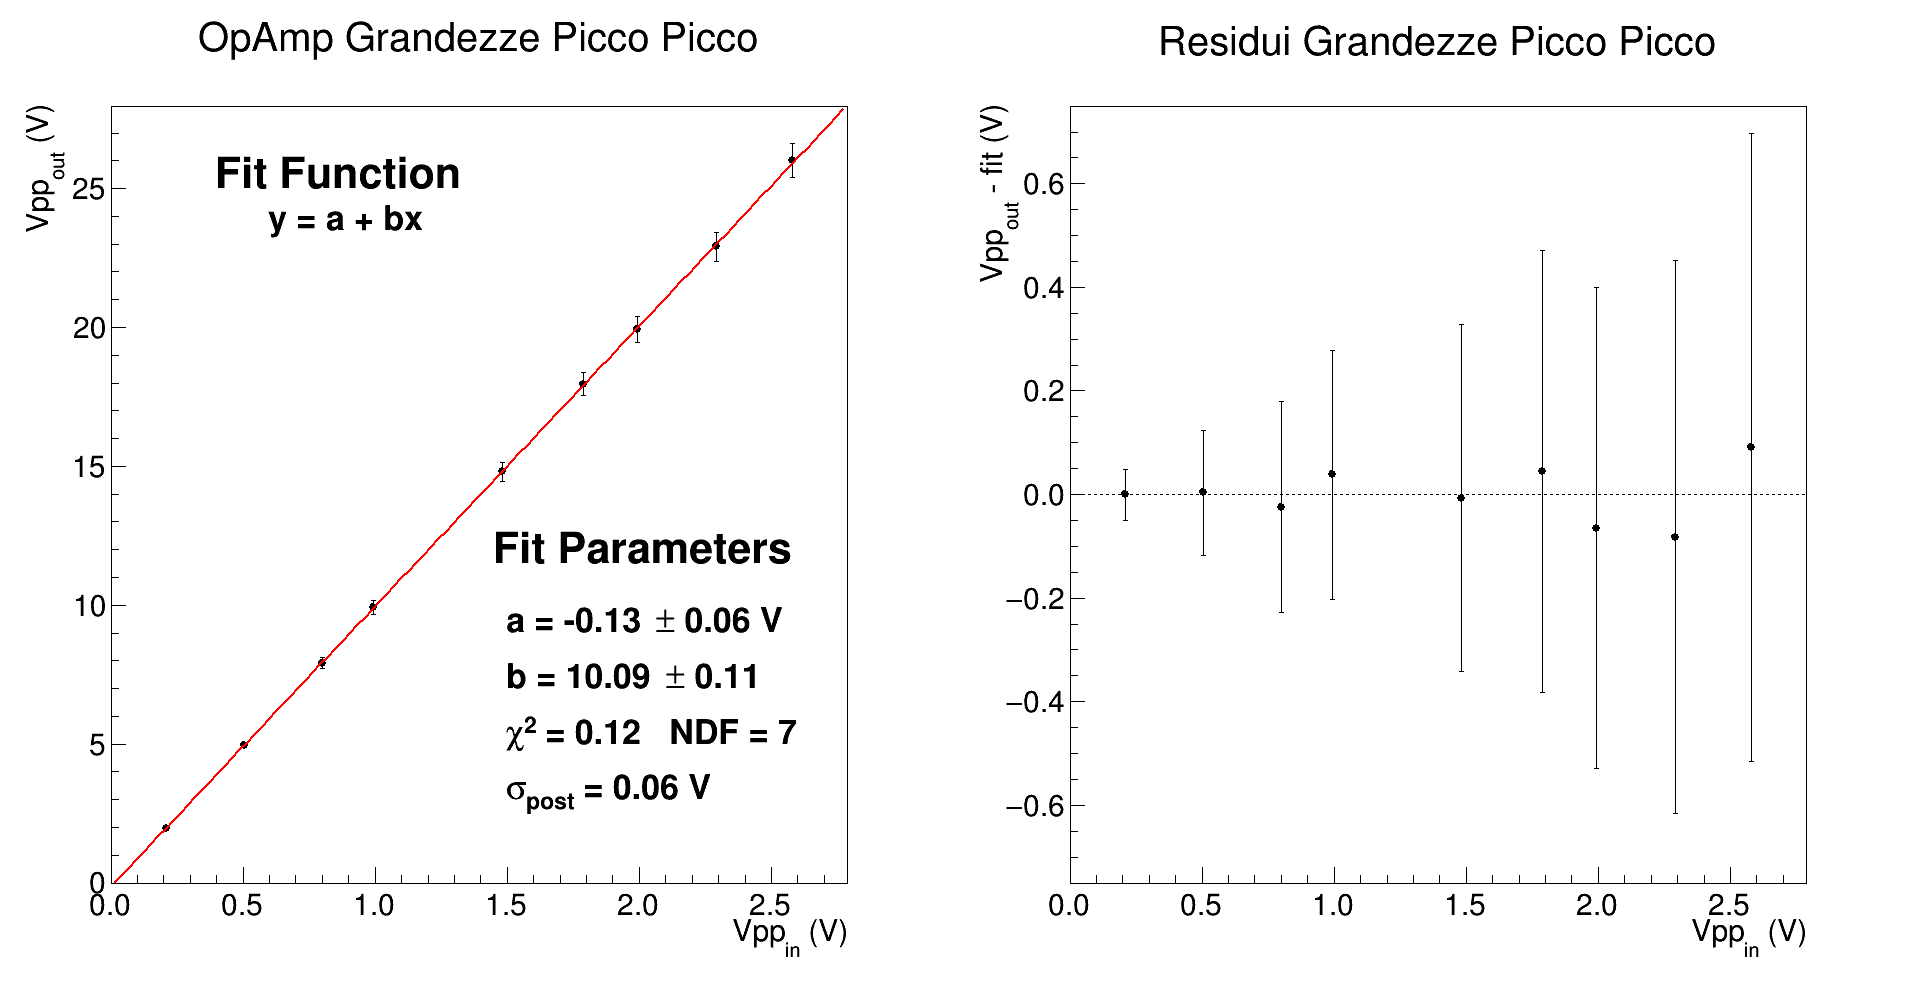
\includegraphics[width=\linewidth]{../Plots/Report_Plots/opamp_plot_pp_projected.png}
	\caption{\small A sinistra: grafico rappresentante il dataset delle grandezze picco picco, 
	con relativa retta interpolante e parametri del fit. A destra: grafico dei residui $V_{\text{pp, out}}-\text{fit}$.}
	\label{i:opamp_pp}
\end{figure}
\noindent Si noti ora come, al contrario di quanto ritrovato in \autoref{i:opamp_all_proj}, l'intercetta $a$ risulti
essere scarsamente compatibile con zero: essa, infatti, assume proprio il valore dello sfalsamento $d$ tra i due
campioni di misure. Il coefficiente angolare $b$, invece,è perfettamente in linea con quanto ottenuto considerando i
dataset sepratamente e, di consegueza, conforme alle aspettative teoriche. Quanto appena riportato fornisce dunque
un'ulteriore conferma all'ipotesi di offset/shift verticale tra i due campioni che, essendo questo costante per tutte le
misure, si riesce ad eliminare studiando le grandezze picco picco. Nel grafico dei residui, questo si tradice
nell'assenza dell'andamento patologico ricontrato in \autoref{i:opamp_all_proj}: come si può osservare, infatti, i punti
sono tutti ben distribuiti attorno allo zero, abbondantemente compreso entro la barra d'errore dei dati. L'errore a
posteriori, inoltre, risulta essere appena maggiore dell'incertezza associata al primo punto, mentre diventa
notevolmente inferiore per i dati successivi. Tale valore di $\sigma_{\text{post}}$ è indice di una buona ditribuzione
delle misure attorno alla retta suggerendo, assieme all'andamento dei residui, una soddisfacente linearità
dell'amplificatore operazionale. Il valore estremamente ridotto del $\chi^2$, invece, non permette nè di rigettare
l'ipotesi di linearità, nè di poterla confermare (diverso se il $\chi^2$ fosse stato molto grande). Altri
possibili indicatori, come il coefficiente di correlazione e la $t$ di Student non si ritengono, in questo caso,
significativi.


%-------------------------------------------------------------------------------------------------------------------------------------------
%	CONFRONTO STIME DI G
%-------------------------------------------------------------------------------------------------------------------------------------------

\subsubsection{Confronto tra Stime di G}

Si vuole ora esporre e confrontare le stime dell'amplificazione $G$ del circuito, ricavate nel corso dell'analisi
riportata nella sezione precedente, rappresentando tali stime in \autoref{i:opamp_comp}. Il primo punto a sinistra (1)
corrisponde alla stima teorica di $G$, ottenuta in \autoref{e:guadagno} utilizzando le misure dirette della rete
resistiva del circuito. Il secondo ed il terzo punto (2) (3) corrispondono invece alle stime ottenute interpolando
separatamente il campione di massimi ed il campione di minimi. Queste presentano rispettivamente una compatibilità
$\lambda_{\text{MAX}}=1.3$ e $\lambda_{\text{MIN}}=0.2$ con la stima teorica (1) e una compatibilità $\lambda=0.7$ tra
loro. Nonostante (1) ed il valore ottenuto analizzando il campione di minimi si trovino in

\begin{wrapfigure}{L}{0.5\textwidth}
	\centering
	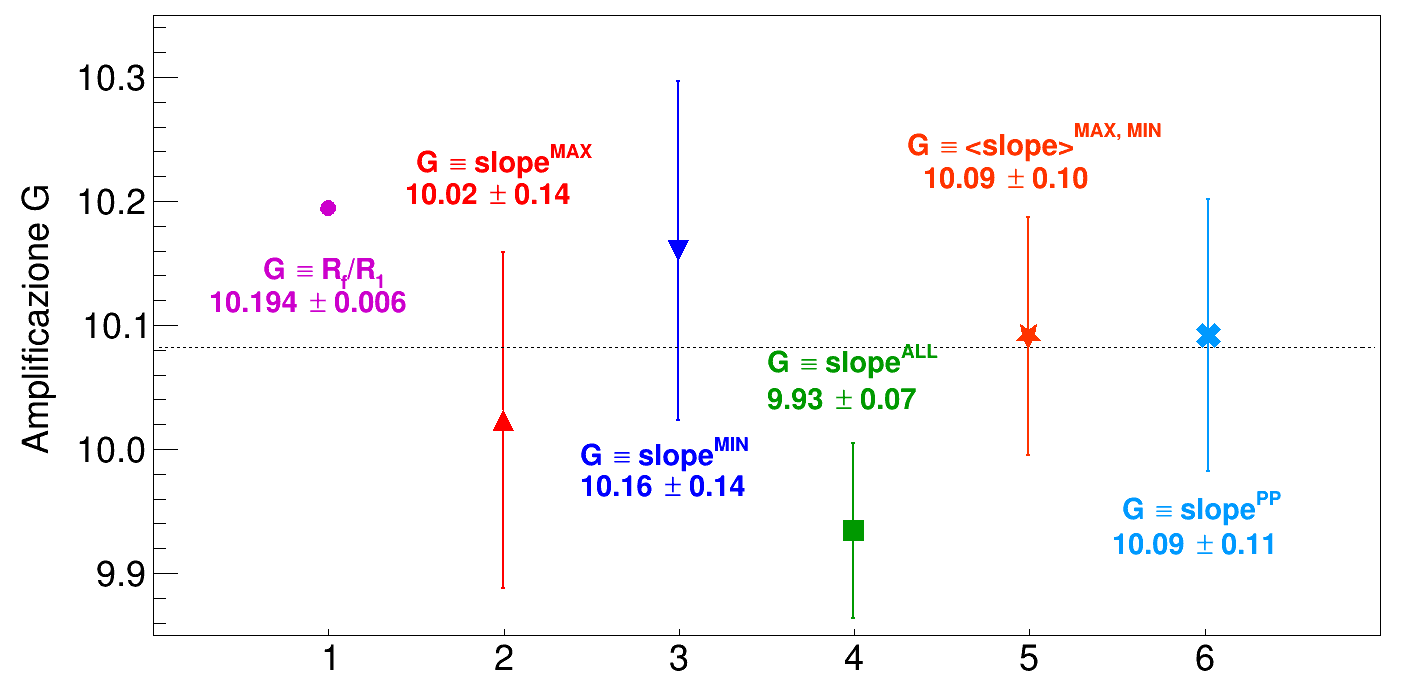
\includegraphics[width=0.5\textwidth]{../Plots/Report_Plots/opamp_comp_BIG.png}
	\caption{\footnotesize Stime di G. Da sinistra: 1) partendo dalle misure dirette delle resistenze; 2) come
	coefficiente angolare del dataset di massimi; 3) come coefficiente angolare del dataset di minimi; 4) come
	coefficiente angolare del dataset unificato; 5) come media pesata di 2 e 3; 6) come coefficiente angolare del
	dataset delle grandezze picco picco.}
	\label{i:opamp_comp}
\end{wrapfigure}

\noindent eccellente accordo, non si considera (3) come miglior stima dell'amplificazione $G$. Si preferisce, infatti,
fornire una stima che tenga conto di tutte le misure acquisite in laboratorio e non solo la metà corrispondente ai
minimi. Il quarto punto, dunque, rappresenta quanto ottenuto interpolando il campione unificato di massimi e minimi. É
piuttosto evidente come questa si discosti dalle rimanenti: come esposto in \autoref{s:pre} tale stima risente di una
sistematica di offset/shift verticale tra i due campioni e si preferisce quindi non prenderla in considerazione. Il
quinto punto rappresenta poi la media pesata di (2) e (3): si vuole far notare come questa sia in perfetto accordo con
(6), ovvero il coefficiente angolare del campione di grandezze picco picco ($\lambda=0.01$ tra media pesata e slope
grandezze picco picco). Si deduce, allora, che eliminando la sistematica presente tra i due dataset si trovino risultati
consistenti e conformi alle aspettative ($\lambda = 0.9$ tra media pesata o slope grandezze picco picco con le
previsioni teoriche). Si assume, in ogni caso, che l'errore sull'amplificazione $G$ sia sottostimato a causa della
correlazione delle incertezze. In conlcusione, si preferisce la stima (6) ottenuta dalle grandezze picco picco, in
quanto presenta un errore relativo leggermente maggiore rispetto alla media pesata (5).


%-------------------------------------------------------------------------------------------------------------------------------------------
%	CIRCUITO DERIVATORE
%-------------------------------------------------------------------------------------------------------------------------------------------

\section{Filtro Attivo - Circuito Derivatore}
Ci si propone ora di studiare il comportamento \textit{in frequenza} di un circuito simile a quello schematizzato in
\autoref{i:opamp_circuit}, con l'aggiunta di un condensatore $C_{1}$ in serie alla resistenza $R_{1}$: questo lo rende
dunque un filtro (attivo, in quanto è sempre presente l'amplificatore operazionale) passa alto, derivatore a basse
frequenze. Si vuole, in particolare, stimare la frequenza di taglio $f_{\text{t}}$ del circuito.

%-------------------------------------------------------------------------------------------------------------------------------------------
%	CONFIGURAZIONE SPERIMENTALE
%-------------------------------------------------------------------------------------------------------------------------------------------

\subsection{Configurazione Sperimentale}
La capacità aggiunta è pari a $C_{1} = 0.977 \pm 0.017 \,\si{n\farad}$ (misurata direttamente utilizzando il multimetro
digitale Metrix a fondo scala $1\,\si{n\farad}$). Vengono poi utilizzate le stesse impostazioni riportate in
\autoref{s:guadagno} per quanto riguarda generatore di funzioni ed oscilloscopio. Inizialmente si configura il
generatore di funzioni in modo da erogare un'onda triangolare di ampiezza $1\,\si{\volt}$ e frequenza $1\,\si{\kHz}$ al
fine di verificare il comportamento derivatore del circuito. Successivamente, per lo studio della risposta in frequenza,
si utilizza un'onda sinusoidale di ampiezza $1\,\si{\volt}$ picco picco e frequenza variabile tra $100\,\si{\Hz}$ e
$1\,\si{\MHz}$. Nel dominio delle frequenze, il modulo della funzione di trasferimento
$H=\left|V_{\text{out}}/V_{\text{in}}\right|$ risulta essere
\begin{align}
	H(\omega) &= \frac{R_{\text{f}}}{R_{1}}\frac{\omega}{\sqrt{\omega^2+\omega_0^2}} & \text{con}\,\,\,\, \omega_{0}&=\frac{1}{R_{1}C_{1}}
\end{align}
\noindent Si noti allora che il termine $\frac{R_{\text{f}}}{R_{1}}$ è esattamente l'amplificazione $G$ del circuito
studiato in \autoref{s:opamp}, mentre il termine $\frac{\omega}{\sqrt{\omega^2+\omega_0^2}}$ è tipico di un filtro
passivo passa alto. Ci si aspetta allora che, considerando entrambi i termini, il circuito si comporti come derivatore a
basse frequenze e che si ottenga il massimo guadagno, pari a $G$, al tendere di $\omega\rightarrow\infty$. Avendo quindi
misurato le componenti circuitali direttamente con il multimetro, e ricordando che $\omega=2\pi f$, la stima teorica del
massimo guadagno $G$ è già stata esplicitata in \autoref{e:guadagno}, mentre ci si aspetta una frequenza di taglio
\begin{align}\label{e:diff_f_th}
	f_{\text{t}}&=\frac{1}{2\pi R_{1}C_{1}}=20.1 \pm 0.3 \,\si{k\Hz} & 
	\text{con\,\,\,\,}\sigma_{f_{\text{t}}}&=\frac{1}{2\pi}\sqrt{	\left(\frac{1}{C_{1}R_{1}^2}\right)^2\sigma_{R_{1}}^2	+
																	\left(\frac{1}{C_{1}^2R_{1}}\right)^2\sigma_{C_{1}}^2   }																	
\end{align}


%-------------------------------------------------------------------------------------------------------------------------------------------
%	ACQUISIZIONE MISURE
%-------------------------------------------------------------------------------------------------------------------------------------------

\subsection{Acquisizione Misure}

Per studiare la risposta in frequenza del circuito, si acquisiscono le misure di tensione picco picco sia del segnale in
ingresso sia del segnale in uscita facendo variare la frequenza dell'onda sinusoidale erogata dal generatore partendo da
$100\,\si{\Hz}$ fino a $1\,\si{\MHz}$. Inizialmente, viene effettuata un'acquisizione preliminare al fine di individuare
gli intervalli di frequenza più interessanti, quali l'intorno della frequenza di taglio e l'intorno del massimo di
amplificazione. Si trova infatti che quest'ultimo non viene assunto al tendere della frequenza verso valori sempre
maggiori ma, piuttosto, si ha un fenomeno di attenuazione del segnale in uscita oltre una certa frequenza "di massimo".
Campionando poi in modo più fitto tali intervalli di frequenze si riesce a fornire una stima "sperimentale" della massima
amplificazione $G_{\text{sper}}\approx 9.8$ e della frequenza di taglio $f_{\text{t, sper}}\approx 19.7\,\si{k\Hz}$.


%-------------------------------------------------------------------------------------------------------------------------------------------
%	DATI E ANALISI
%-------------------------------------------------------------------------------------------------------------------------------------------

\subsection{Dati e Analisi}

Si vuole inizialmete verificare il comportamento derivatore del circuito sfruttando l'onda triangolare in ingresso.
Successivamente invece si vogliono rappresentare le misure acquisite sperimentalmente sotto forma di grafico di Bode:
dallo studio di questo si vogliono poi estrarre informazioni di carattere generale sui dati e fornire una stima della
frequenza di taglio del circuito.


%-------------------------------------------------------------------------------------------------------------------------------------------
%	COMPORTAMENTO DERIVATORE
%-------------------------------------------------------------------------------------------------------------------------------------------

\subsubsection{Comportamento Derivatore}

Sfruttando l'onda triangolare in ingresso, come anticipato, si vuole ora verificare il comportamento 

\begin{wrapfigure}{R}{0.4\textwidth}
	\centering
	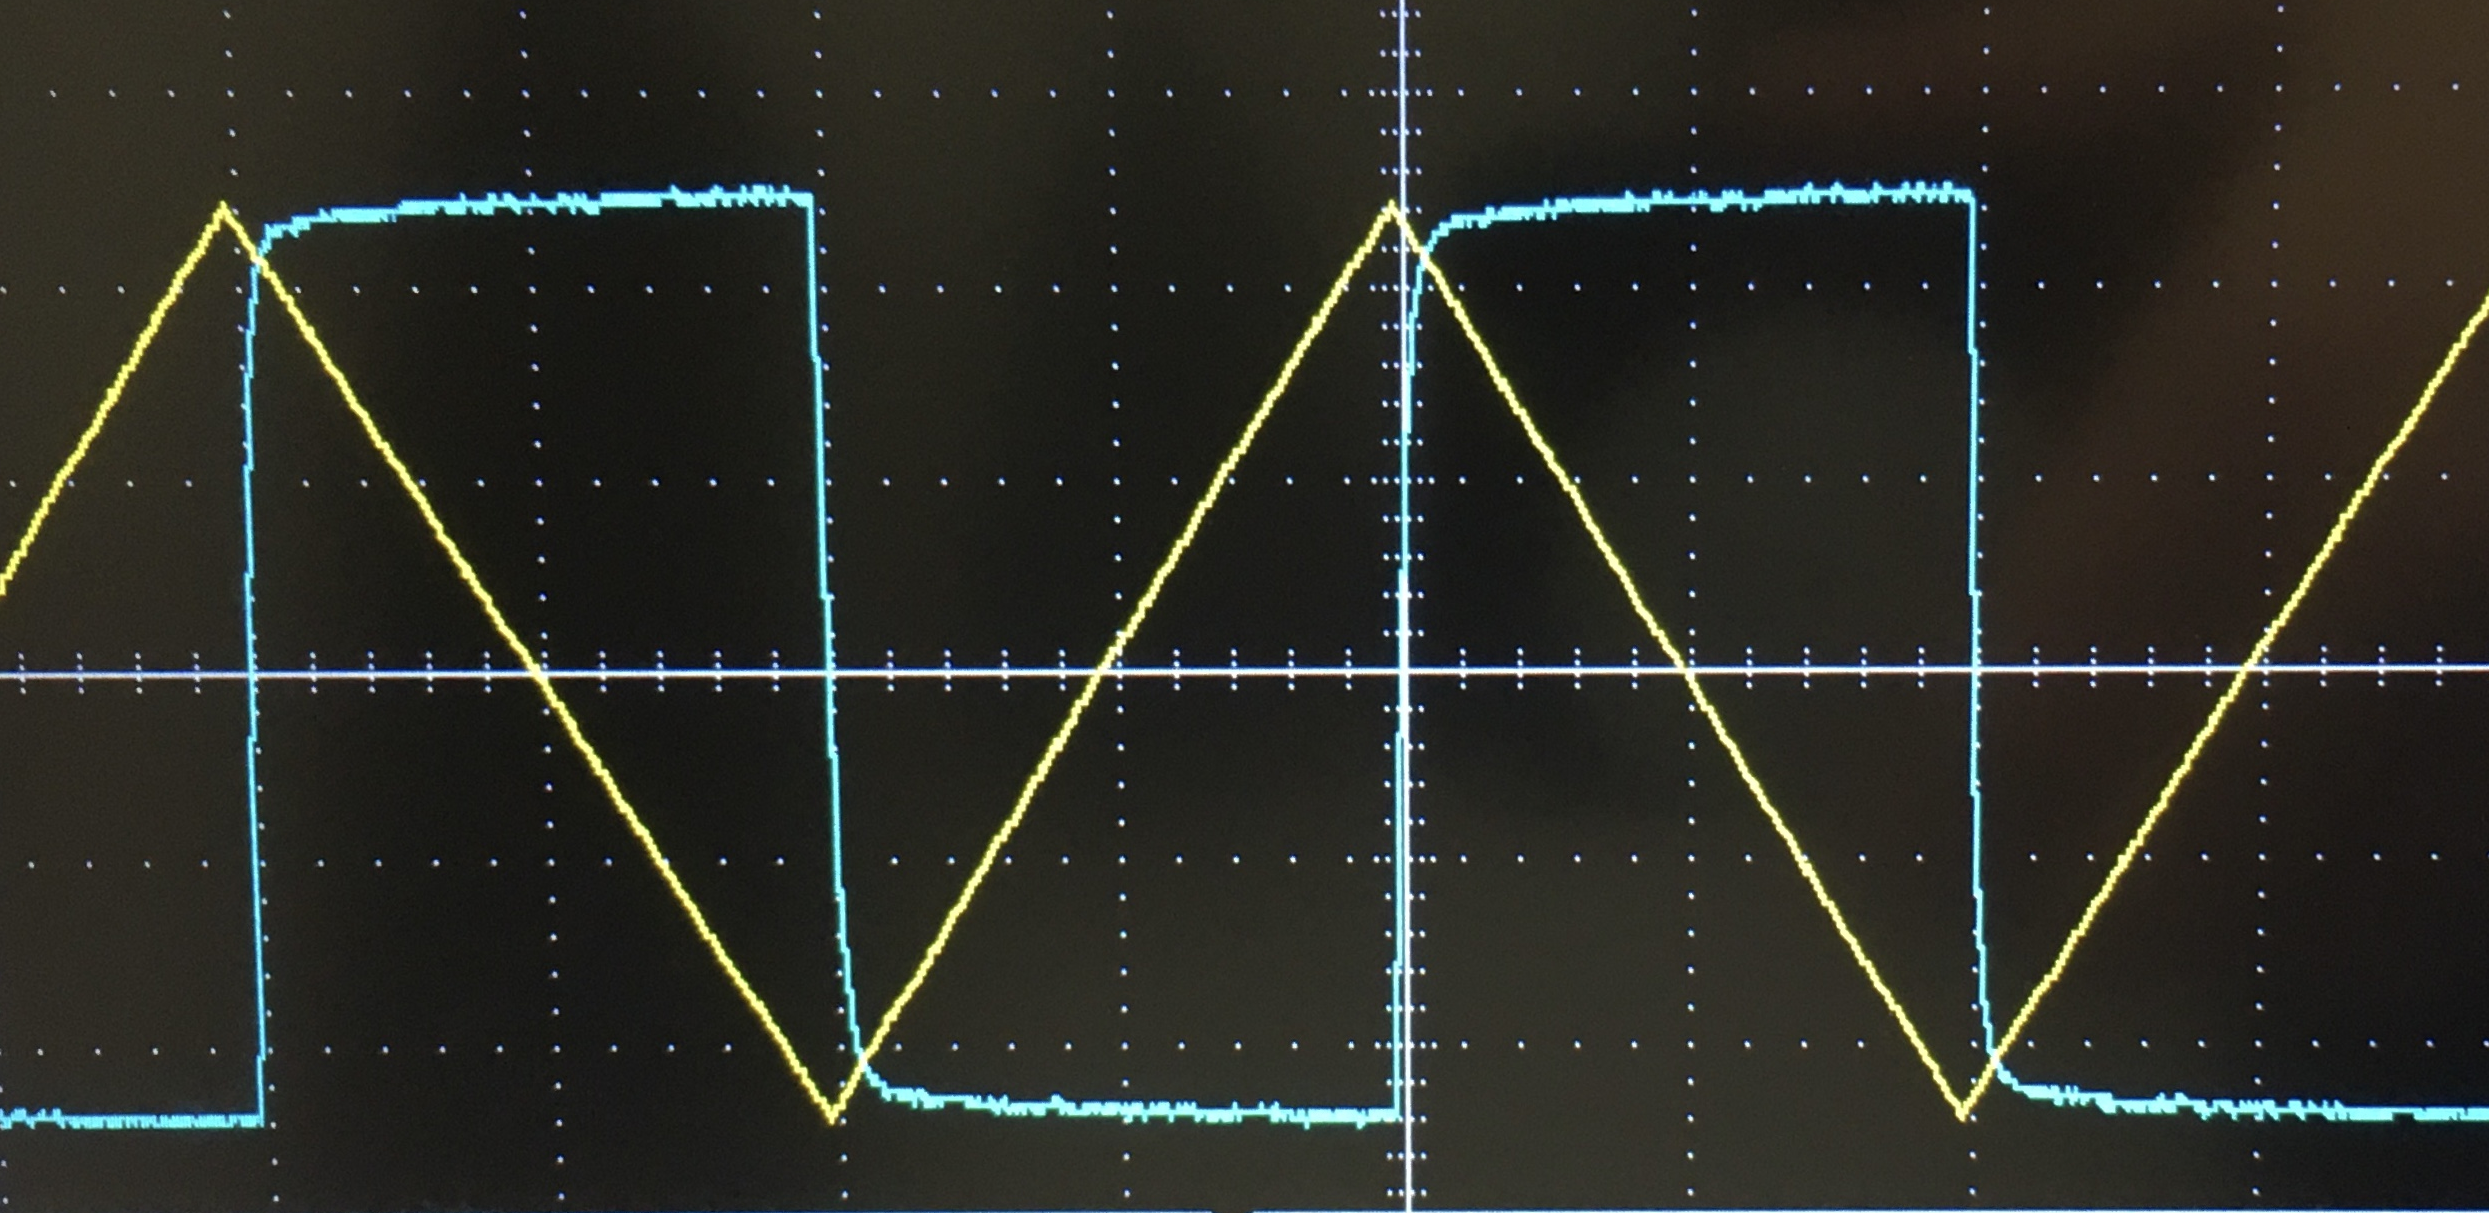
\includegraphics[width=0.4\textwidth]{../Plots/Report_Plots/diff_osc_pic.png}
	\caption{\small Display dell'oscilloscopio: onda triangolare in input e onda quadra in output.}
	\label{i:diff_pic}
\end{wrapfigure}

\noindent derivatore del circuito. Ricordando allora che il segnale derivato della salita lineare è la funzione a
gradino, per l'onda triangolare in input ci si aspetta un'onda quadra in output. In \autoref{i:diff_pic} è riportato il
display dell'oscilloscopio, nel quale si può osservare la traccia del segnale in ingresso (in giallo) e la traccia del
segnale in uscita (in azzurro). Per le considerazioni appena riportate, il comportamento derivatore del circuito è
dunque verificato. Si osserva, inoltre, che l'onda quadra non risulta essere perfetta: questo è dovuto principalmente al
fatto che l'onda triangolare in ingresso possiede una frequenza di $1\,\si{\kHz}$. Essendo il circuito un filtro passa
alto, il comportamento derivatore risulta essere più accentuato a basse frequenze. Ci si aspetta dunque che riducendo la
frequenza dell'onda triangolare in ingresso la forma dell'onda quadra migliori, mentre l'ampiezza diminuisca.


%-------------------------------------------------------------------------------------------------------------------------------------------
%	THEBODE
%-------------------------------------------------------------------------------------------------------------------------------------------

\subsubsection{Grafico di Bode}
Si vogliono ora rappresentare le misure acquisite sperimentalmente sfruttando un grafico di Bode. Date le misure di
tensione $V_{\text{in}}$ e $V_{\text{out}}$, dunque, viene calcolata la funzione di trasferimento $H$, alla quale viene
associata un'incertezza $\sigma_{H}$ data da
\begin{align}\label{e:diff_err}
	H&=\frac{V_{\text{out}}}{V_{\text{in}}} & 
	\sigma_{H}&= H \sqrt{	
						\left(	\frac{	\sigma_{\text{L}}\times V_{\text{in}}/\text{div}	}{	V_{\text{in}}	}	\right)^2	 + 
						\left(	\frac{	\sigma_{\text{L}}\times V_{\text{out}}/\text{div}	}{	V_{\text{out}}	}	\right)^2 +	
						2\left(	\frac{	\sigma_{\text{k}}	}{	k	}	\right)^2 }	
\end{align}
\noindent dove $\sigma_{\text{L}}=0.04$ rappresenta l'incertezza di lettura associata all'oscilloscopio, i termini
$V_{\text{in}}/\text{div}$ e $V_{\text{out}}/\text{div}$ corrispondono al numero di volt per divisione per il canale di
acquisizione rispettivamente del segnale in ingresso e del segnale in uscita, mentre $\sigma_{\text{k}}=1.5\%$
rappresenta l'incertezza di guadagno associata all'oscilloscopio: quest'ultima viene considerata in quanto le misure non
sono state acquisite utilizzando un'unica scala e, inoltre, sono state acquisite utilizzando due diversi canali. Si
assume poi che $k$ sia mediamente pari all'unità e che l'incertezza sulla frequenza dell'onda erogata dal generatore sia
trascurabile. Si rappresenta allora in \autoref{i:diff_bode} il grafico di Bode delle misure acquisite assieme ai punti
ottenuti attraverso una simulazione Spice della risposta del circuito. \newpage
\begin{figure}[H]
	\centering
	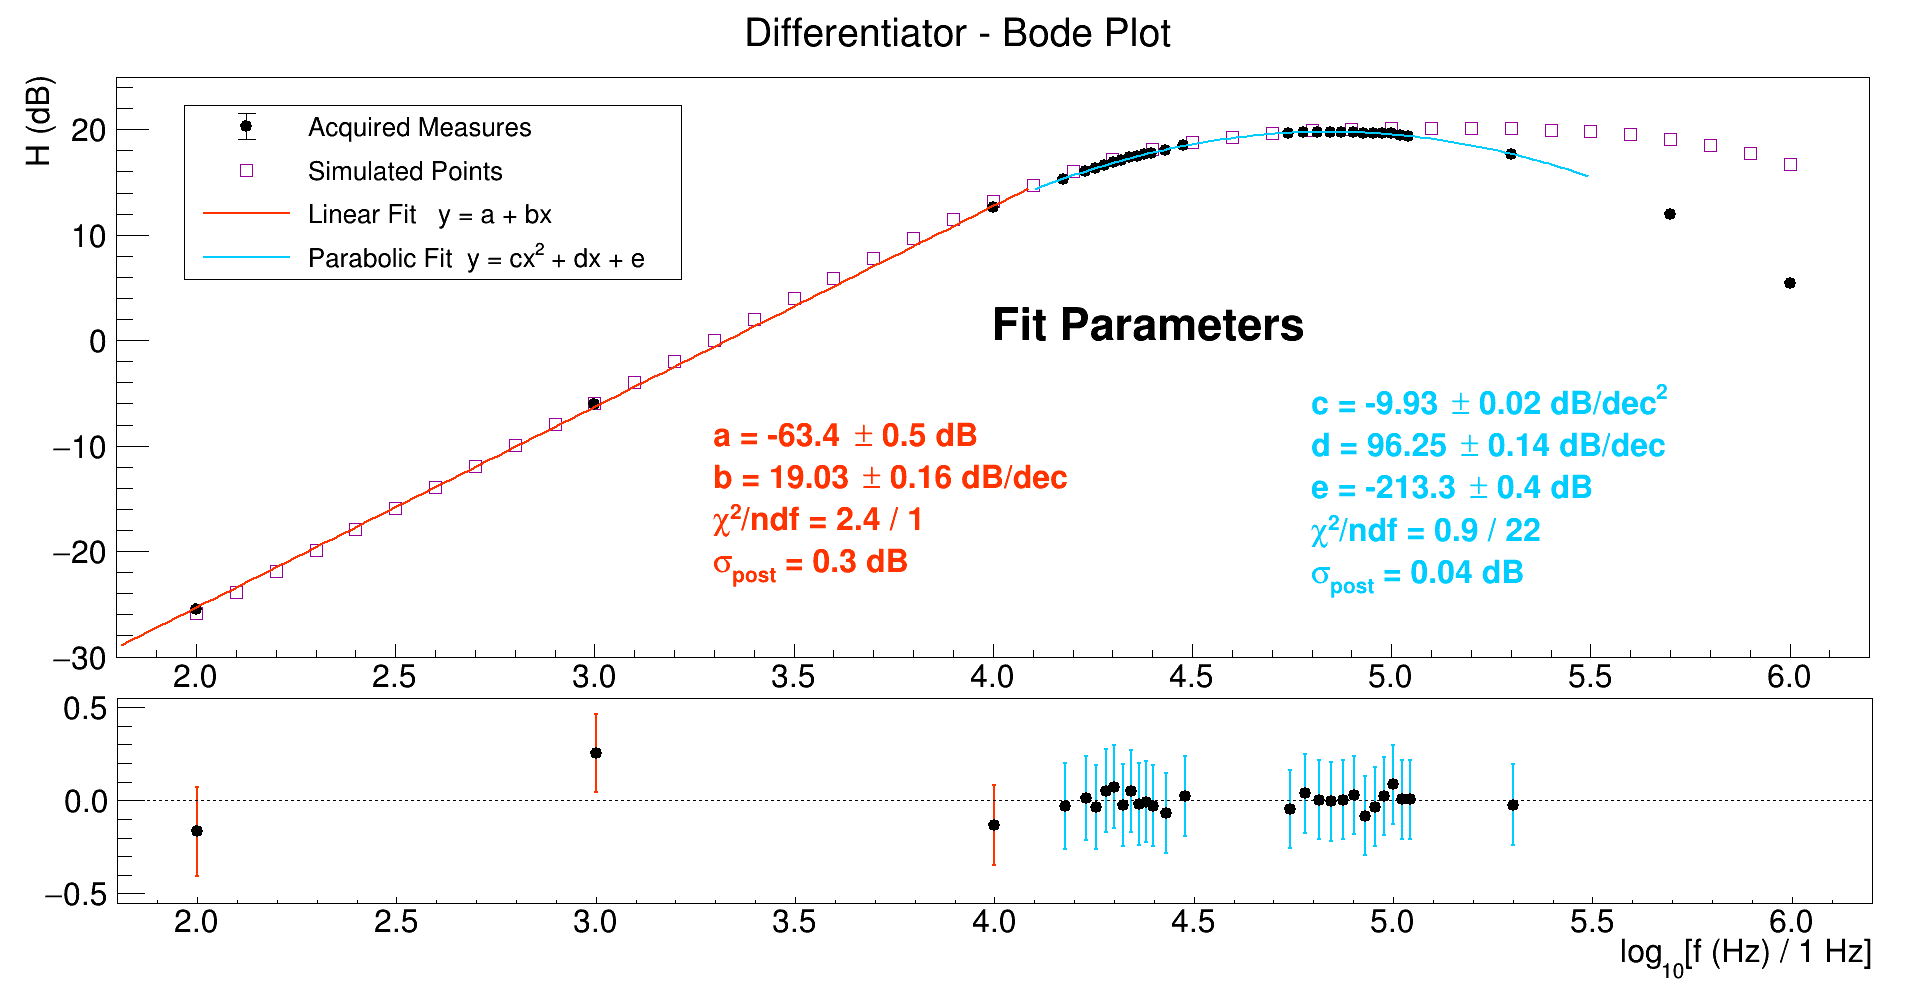
\includegraphics[width=\linewidth]{../Plots/Report_Plots/diff_bode.png}
	\caption{\small Grafico di Bode delle misure sperimentali e dei dati simulati. Le misure sperimentali vengono
	interpolate con una retta $y = a + bx$ e con una parabola $y = cx^2+dx+e$. Vengono mostrati anche i residui, 
	rispettivamente per la retta e per la parabola.}
	\label{i:diff_bode}
\end{figure}
\noindent Si noti inizialmente che nel grafico sono riportate due interpolazioni. La prima, lineare, è
caratterizzata dalla traccia arancione: per questo fit sono state prese in considerazione unicamente le prime tre
misure in quanto, ampliando ulteriormente l'intervallo di interpolazione, sarebbero stati considerati punti che non
rispettano il trend lineare. La seconda, invece, è un fit parabolico (traccia azzurra) ristretto all'intorno del
massimo della funzione di trasferimento. Confrontando le misure sperimentali con la simulazione Spice, la zona
lineare sulla sinistra presenta un accordo soddisfacente tra le due. Lo stesso vale nell'intorno della frequenza di
taglio. Spostando l'attenzione verso la zona destra del grafico, invece, si vede chiaramente un effetto di
attenuazione della funzione di trasferimento, tipico di un filtro passa banda piuttosto che di un passa alto. Questo
comportamento, infatti, si trova in disaccordo con 

	\begin{wrapfigure}{R}{0.5\textwidth}
		\centering
		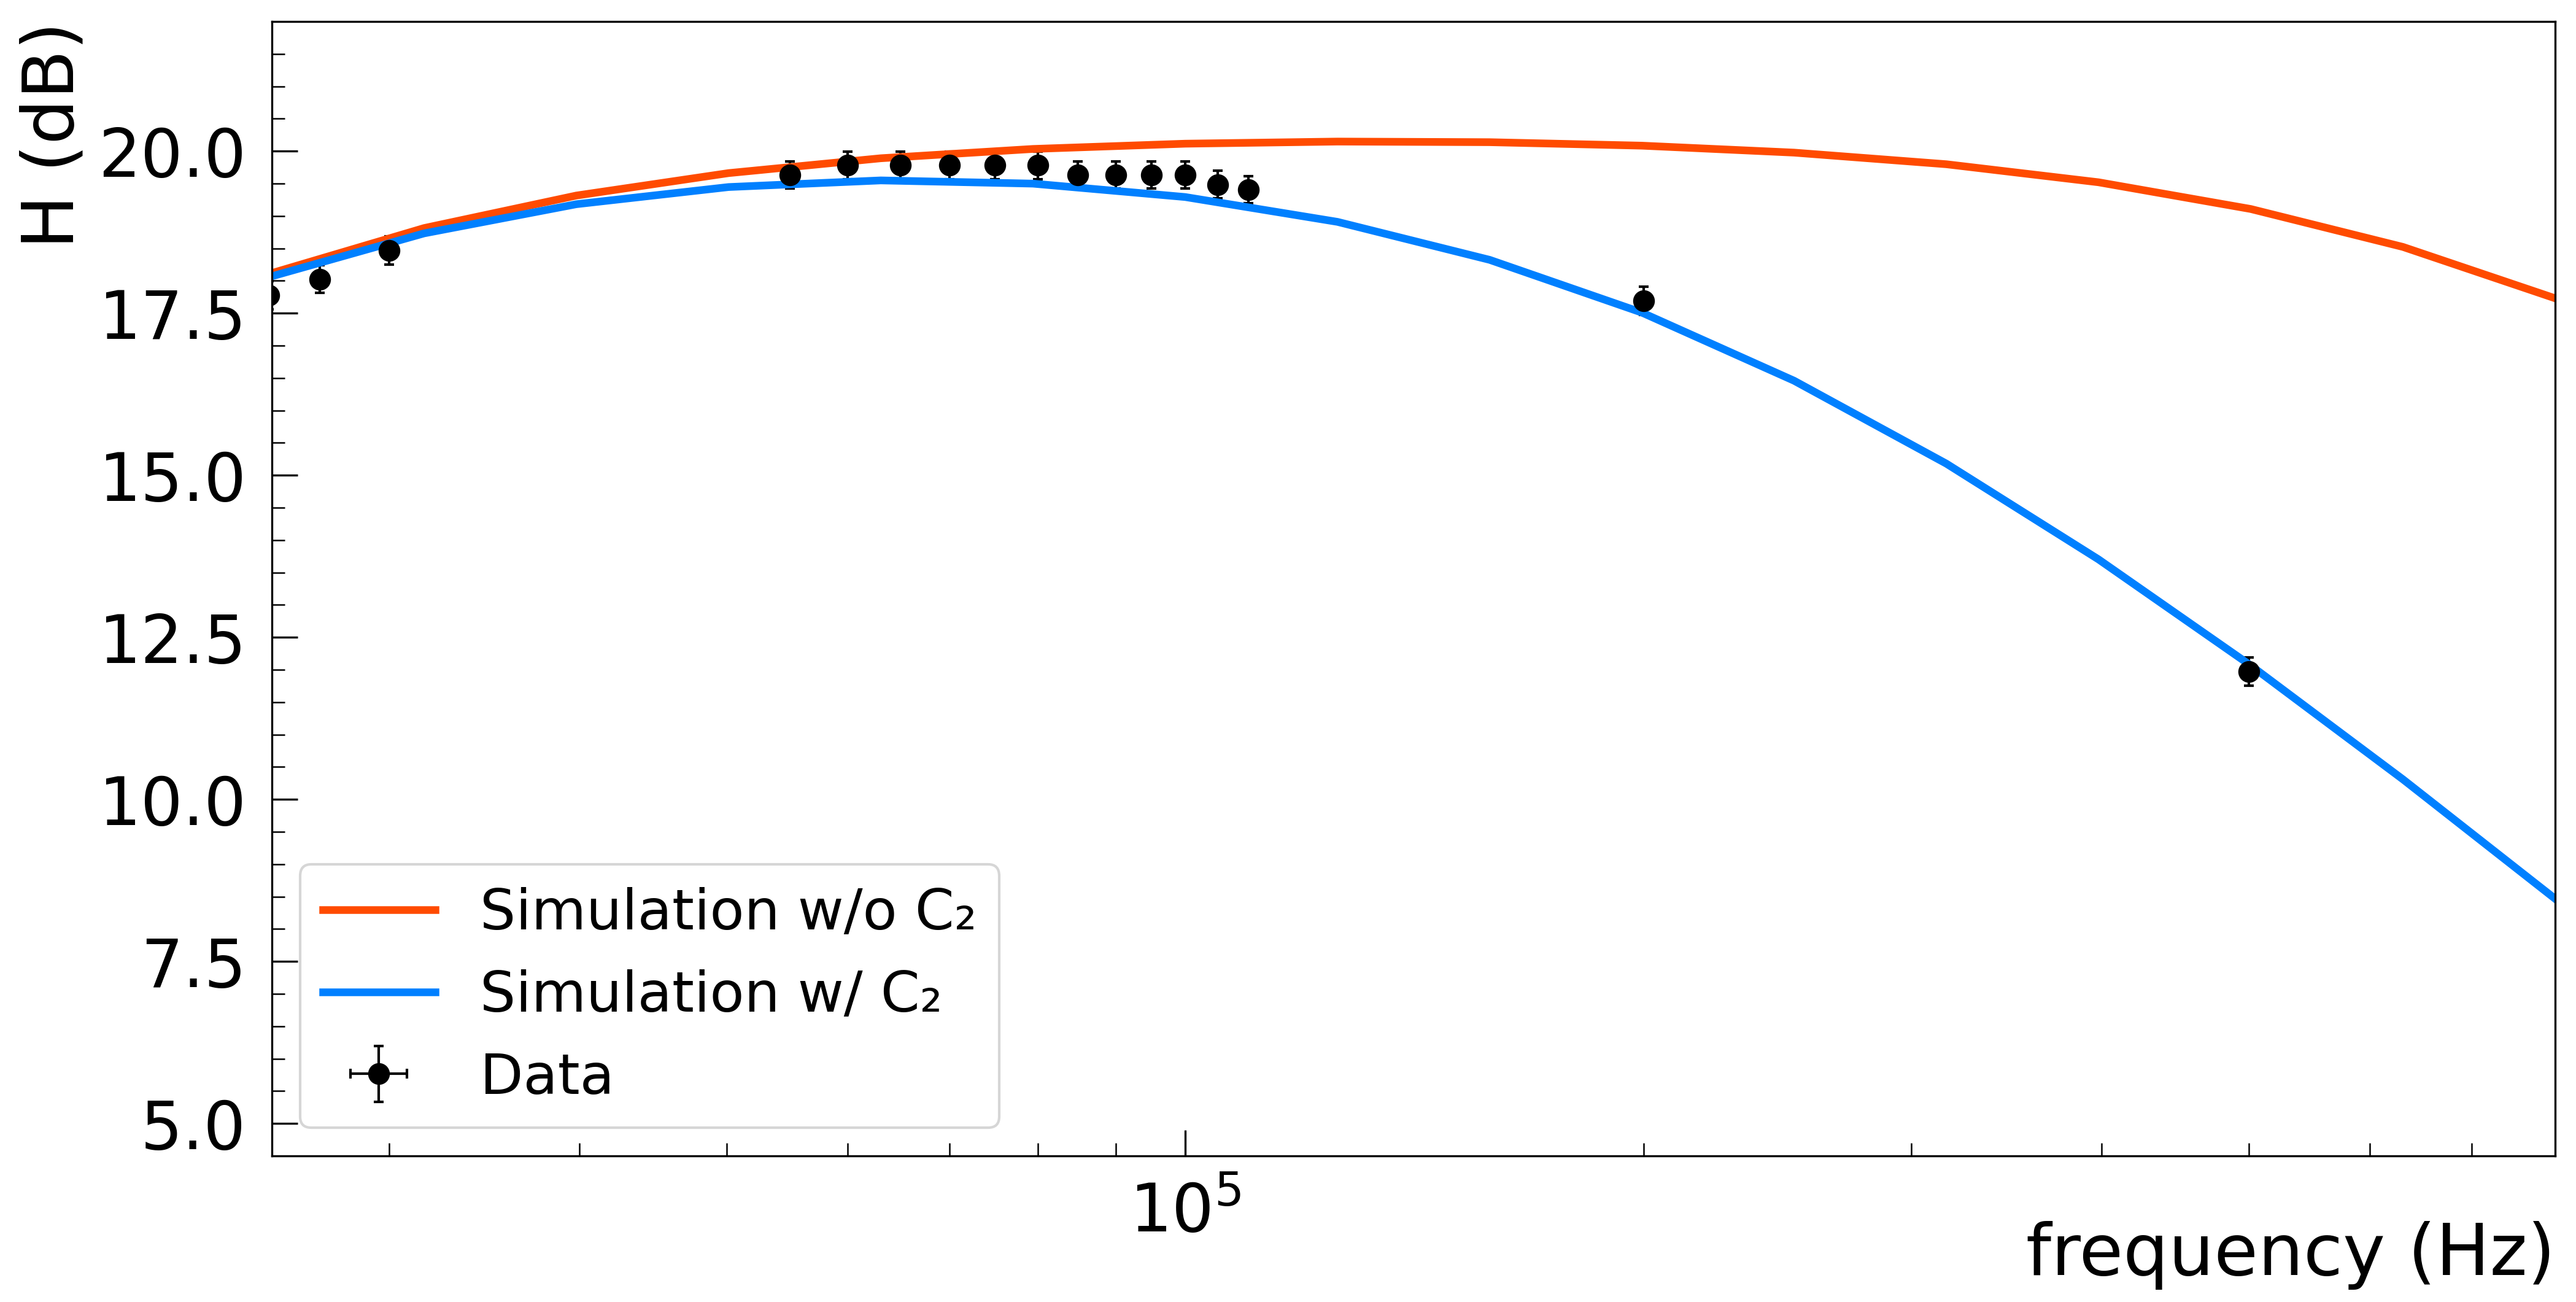
\includegraphics[width=0.5\textwidth]{../Plots/Report_Plots/diff_sim_comp.png}
		\caption{\small Confronto misure-simulazioni.}
		\label{i:diff_sim_comp}
	\end{wrapfigure}
	
\noindent la simulazione Spice del circuito ed è, con buona probabilità, indice della presenza di una capacità (non
considerata nella simulazione) in parallelo al circuito: breadboard, cavi, sonde, oscilloscopio. Effettuando
un'ulteriore simulazione, aggiungendo una capacità $C_{2}=7\,\si{\pF}$ in parallelo alla resistenza di feedback
$R_{\text{f}}$, si trova un notevole miglioramento nell'accordo tra punti simulati e misure sperimentali: questo
conferma dunque che l'effetto di attenuazione della funzione di trasferimento del circuito è dovuto a dei contributi
capacitivi non trascurabili posti in parallelo ad esso. In \autoref{i:diff_sim_comp} è messo in evidenza questo
confronto tra i dati sperimentali e quelli simulati, sia trascurando la capacità $C_{2}$ (in arancione) sia invece
tenendone conto (in azzurro). Si procede ora nella ricerca della frequenza di taglio $f_{\text{t}}$ del circuito: la
strategia per la stima di tale frequenza è la seguente. Inizialmente si stima il massimo della funzione di
trasferimento come vertice della parabola e si associa a tale valore una retta orizzontale
$y=H_{\text{max}}=19.79\pm 0.05\,\text{dB}$, dove nel computo dell'errore sono state tenute in considerazione le
opportune covarianze tra i parametri della parabola. Si calcola poi il punto di intersezione con la retta  $y=a+bx$
in arancione: la coordinata $x$ di tale punto fornisce quindi una stima della frequenza di taglio
$f_{\text{t}}=4.370 \pm 0.017\,\text{dec}$ (anche in questo caso nel computo dell'errore è stata considerata la
covarianza tra i parametri $a$ e $b$ della retta). Convertendo quanto trovato in Hertz, la frequenza di taglio così
stimata risulta essere $f_{\text{t}}=23.4 \pm 0.9\,\si{k\Hz}$. Tale valore è però incompatibile sia con le
aspettative teoriche sia con quanto trovato sperimentalmente, seppur in modo approssimativo. Si ipotizza dunque che
la causa possa essere il leggero disaccordo tra il coefficiente angolare della retta arancione $b = 19.03\pm
0.16\,\text{dB/dec}$ e l'aspettativa $b_{\text{th}}=20\,\text{dB/dec}$: sfruttando la strategia riportata sopra,
infatti, una pendenza minore di tale retta si tradurrebbe in un aumento della frequenza di taglio. Nella sezione
successiva allora ci si propone di stimare la frequenza di taglio $f_{\text{t}}$ utilizzando un metodo alternativo
al fine di verificare se questa incompatibilità con le aspettative risulti essere ricorrente.


%-------------------------------------------------------------------------------------------------------------------------------------------
%	FIT LINEARIZZATO
%-------------------------------------------------------------------------------------------------------------------------------------------

\subsubsection{Stima di $\mathbf{f_{\text{t}}}$ in Scala Lineare}

Si considerano ora frequenza e funzione di trasferimento in scala lineare e si effettua un fit del tipo $y = mx + q$ in
uno stretto intorno della frequenza di taglio. Ricordando che la frequenza di taglio è tale da attenuare la funzione di
trasferimento di un fattore $1/\sqrt{2}$, la prima può essere ricavata da
\begin{align}
	\frac{H_{\text{max}}}{\sqrt{2}}&=mx+q & \Longrightarrow & & f_{\text{t}}&=\frac{\frac{H_{\text{max}}}{\sqrt{2}}-q}{m}
\end{align}

\noindent Per effettuare il fit, il contributo di scala presente in \autoref{e:diff_err} non viene considerato in quanto
non altera l'andamento dei residui. Il contributo viene quindi aggiunto in secondo luogo sui parametri
dell’interpolazione, in particolare nel calcolo di $f_{\text{t}}$ come segue
\begin{equation}\label{e:diff_prop}
	\sigma_{f_{\text{t}}}=\sqrt{
		\left(
			\frac{\partial f_{\text{t}}}{\partial m}
			%\frac{q}{m^2}-\frac{H_{\text{max}}}{m^2\sqrt{2}}
		\right)^2\sigma_m^2+
		\left(
			\frac{\partial f_{\text{t}}}{\partial q}
			%-\frac{1}{m}
		\right)^2\sigma_q^2+
		%\left(
		%	\frac{\partial f_{\text{t}}}{\partial H}
		%\right)^2\sigma_{H}^2+
		2\left(
			\frac{H_{\text{max}}}{m\sqrt{2}}
		\right)^2\sigma_k^2+
		2\left(
			\frac{\partial f_{\text{t}}}{\partial m}
			%\frac{q}{m^2}-\frac{H_{\text{max}}}{m^2\sqrt{2}}
		\right)
		\left(
			\frac{\partial f_{\text{t}}}{\partial q}
			%-\frac{1}{m}
		\right)\text{cov}(m,q)
	}
\end{equation}
\noindent dove appunto $\sigma_{\text{k}}=1.5\%$ rappresenta il contributo di scala. Si sceglie allora come
$H_{\text{max}} = 9.76 \pm 0.05$ il valore trovato attraverso il fit parabolico precedente (convertito in scala lineare)
e si ricavano i parametri $m$ e $q$ dal seguente fit nell'intervallo di frequenze 17 - 24 kHz. Si vuole far notare che
in \autoref{e:diff_prop} non è stato considerato il contributo relativo ad $H_{\text{max}}$, in quanto due ordini di
grandezza inferiore rispetto agli altri termini e non modifica in quantità apprezzabile la stima finale dell'errore.
\begin{figure}[H]
	\centering
	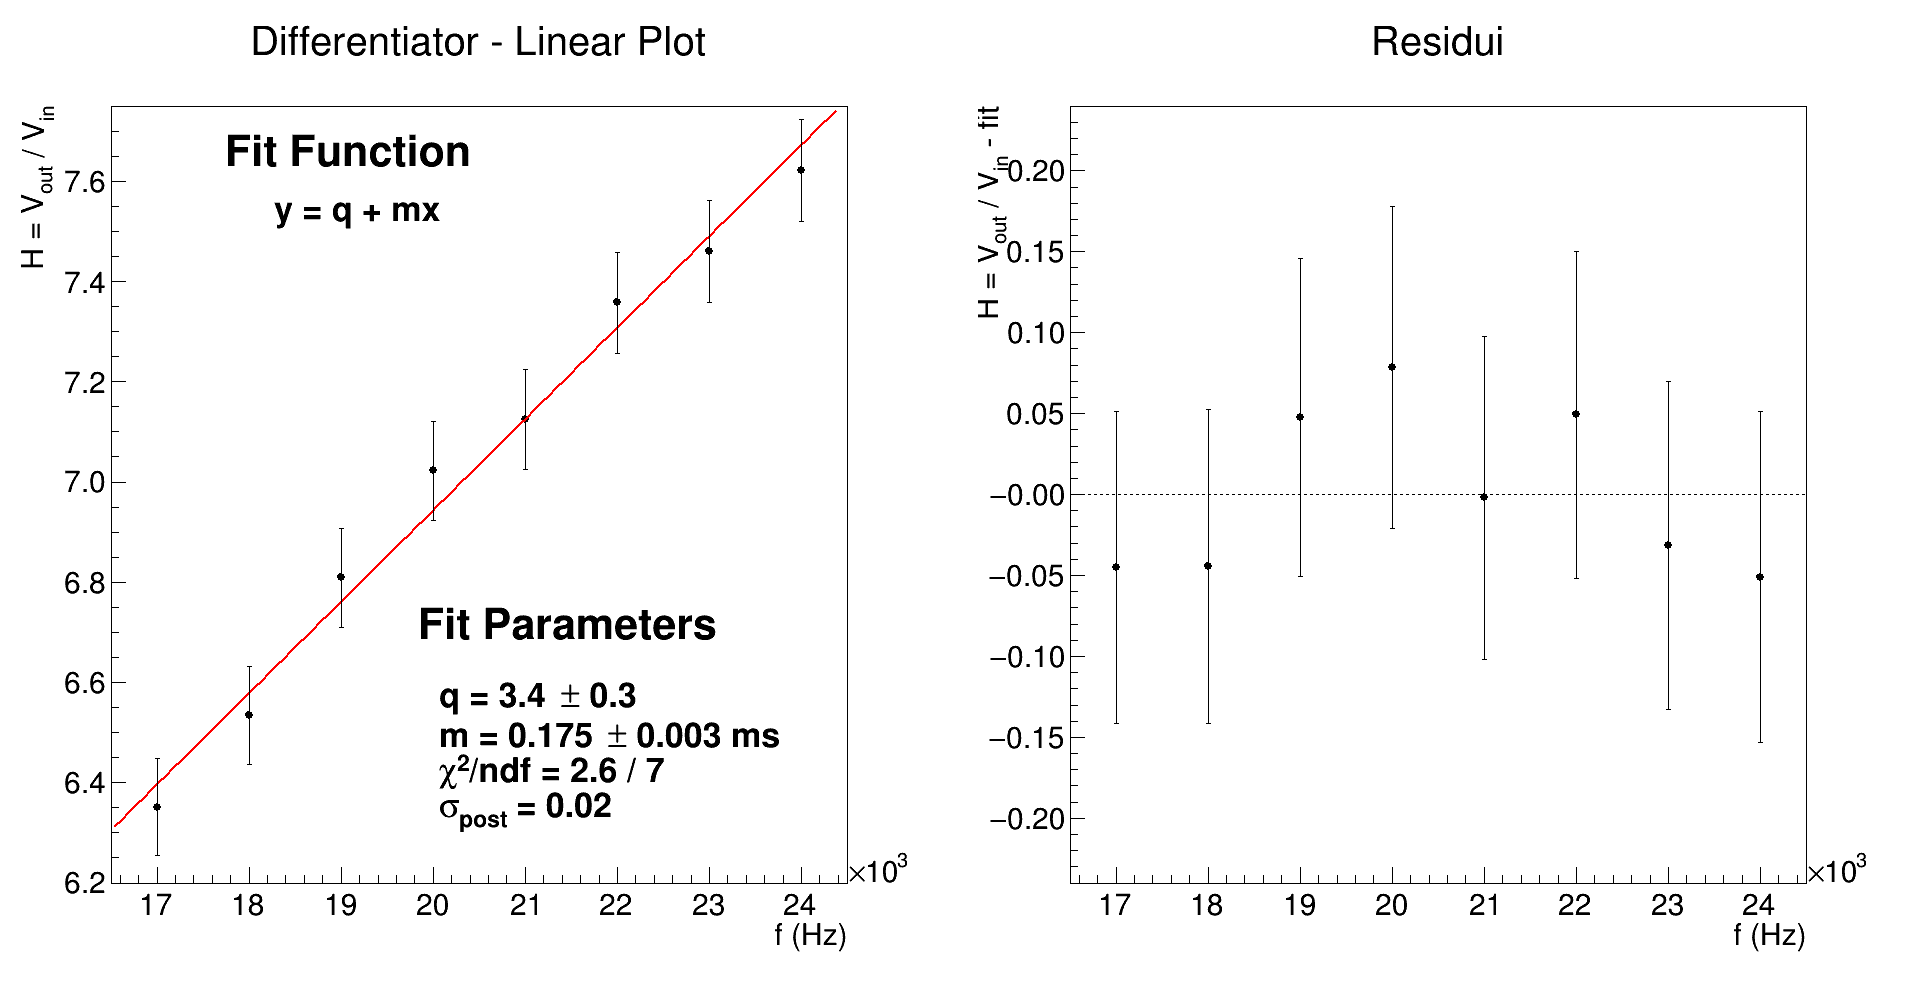
\includegraphics[width=\linewidth]{../Plots/Report_Plots/diff_linear.png}
	\caption{\small Fit lineare delle misure in un intorno della frequenza di taglio e relativo grafico dei residui.}
	\label{i:diff_linear}
\end{figure}
\noindent Si nota immediatamente una leggera tendenza parabolica dell'andamento dei residui, tuttavia, pur avendo
trascurato il contributo di scala nel calcolo delle incertezze, i punti si distribuiscono tutti entro il loro errore. Il
$\chi^2$ risulta in ogni caso compatibile con il suo valore di aspettazione ($\lambda = 1.2$), pur segnalando una
possibile sovrastima dell'errore sulle misure (ipotesi assecondata anche dall'errore a posteriori, che risulta essere
circa $1/5$ rispetto alle incertezze assegnate ai dati). La stima della frequenza di taglio che si ottiene è, infine,
$f_{\text{t}} = 19.8\pm 0.8\,\si{\kHz}$: questa risulta essere in ottimo accordo con le previsioni teoriche
($\lambda=0.4$) e con quanto trovato sperimentalmente. Di conseguenza, questa si trova essere scarsamente compatibile
con quanto ricavato studiando il grafico di Bode ($\lambda = 3.0$).


%-------------------------------------------------------------------------------------------------------------------------------------------
%	ARDUINO
%-------------------------------------------------------------------------------------------------------------------------------------------

\section{Arduino}
In questa sezione si vuole effettuare una calibrazione della scheda Arduino Due. In particolare, si vuole quantificare
il sampling rate dell'ADC della scheda e determinare la funzione di calibrazione in tensione, ovvero $V = a + b \cdot
\text{ADC}$ dove $V$ è il valore in Volt del segnale, $\text{ADC}$ è la tensione in ADC counts acquisita da Arduino,
mentre $a$ e $b$ sono i parametri di calibrazione. Si ricorda che la scheda in questione presenta un ADC a 12 bit,
ovvero 4096 valori, e l'\textit{operating voltage} caratteristico (ovvero il valore massimo di tensione che può leggere
in input) è $V_{\text{op}}=3.3\,\si{\volt}$.\footnote{\url{https://www.arduino.cc/en/pmwiki.php?n=Main/arduinoBoardDue}}
La più piccola variazione di tensione rilevabile in ADC counts risulta dunque essere circa $0.8\,\si{\mV}$. Ci si
aspetta dunque di trovare una funzione di calibrazione in tensione con un coefficiente angolare attorno a tale valore. 

%-------------------------------------------------------------------------------------------------------------------------------------------
%	SAMPLING RATE 
%-------------------------------------------------------------------------------------------------------------------------------------------

\subsection{Sampling Rate}
Si comincia configurando il segnale di trigger. Si imposta quindi nel canale CH2 del generatore un impulso quadrato di
durata $10\,\si{\us}$, frequenza $1\,\si{k\hertz}$ e altezza $2\,\si{\volt}$ a partire dallo zero. Sul canale CH1 del
generatore, invece, si imposta un'onda quadra di ampiezza $1\,\si{\volt}$ partendo da zero con frequenza
$5\,\si{k\hertz}$. Conoscendo il periodo dell'onda quadra in ingresso ($T=1/f$), il sampling rate viene computato come
$S = N / T = N \, f$ con $N$ il numero di misure acquisite in un periodo. Per calcolare $N$ viene computata la derivata
numerica della forma d'onda: questa presenterà dei picchi positivi quando la funzione passa da zero a $1\,\si{\volt}$ e
picchi negativi quando scende da $1\,\si{\volt}$ a zero. Il numero di acquisizioni in un periodo sarà allora il numeri
di punti compresi tra due picchi positivi della funzione derivata. Si trova allora un sampling rate $S = 955000 s^{-1}$,
ovvero 955000 acquisizioni al secondo.


%-------------------------------------------------------------------------------------------------------------------------------------------
%	CALIBRAZIONE IN TENSIONE
%-------------------------------------------------------------------------------------------------------------------------------------------

\subsection{Calibrazione in Tensione}
Si vuole ora verificare la linearità dell'ADC interno alla scheda e stimare i parametri $a$, $b$ della funzione di
calibrazione, in quanto si è interessati a convertire il segnale acquisito da ADC counts in Volt. Si acquisiscono allora
diverse forme d'onda facendo variare la tensione del generatore, avendo cura di misurare il segnale erogato con i
cursori dell'oscilloscopio, in quanto può non essere esattamente uguale a quello nominale indicato dal generatore. Si
rappresentano in grafico i valori di tensione $V$ misurati sperimentalmente contro la media dei punti appartenenti ai
picchi della relativa forma d'onda (si decide di non considerare unicamente il massimo della forma in quanto è possibile
si tratti di una fluttuazione). Per quanto riguarda le incertezze associate ai dati, si associa lungo y l'errore
riportato in \autoref{e:osc} (misure acquisite utilizzando i cursori), mentre si assume che l'incertezza di acquisizione
delle misure di Arduino sia trascurabile rispetto a quella dell'oscilloscopio e non viene quindi considerata.
Effettuando poi un'interpolazione lineare, riportata in \autoref{i:ar_calib}, si ricavano l'offset (cioè quanti Volt
corrispondono allo zero dell'ADC) ed il coefficiente angolare (cioè come scalano i Volt rispetto all'ADC).
Osservando il grafico dei residui, si nota un marcato andamento anomalo dei punti a tensioni maggiori, oltre i
$2\,\si{\volt}$: la scheda, cioè, risponde in modo leggermente diverso a seconda della tensione in ingresso. Questo è,
molto probabilmente, dovuto al circuito di protezione dei pin di ingresso (limitatore di tensione a diodi, utile per
evitare di bruciare la scheda) che ne altera la risposta avvicinandosi a tensioni pericolose. Si prova allora ad
effettuare nuovamente l'interpolazione rimuovendo i punti relativi a tensioni in ingresso maggiori di $2\,\si{\volt}$:
nonostante l'andamento dei residui migliori, anche il primo punto (tensione in ingresso pari a $200\,\si{\mV}$) si trova
essere fuori trend. Si ottengono quindi due zone in cui la linearità dell'ADC risulta essere ottimale: la prima tra
$500\,\si{\mV}$ e $1.8\,\si{\volt}$ (parametri di calibrazione: $a = -0.59 \pm 0.02 \, \si{\V}$ e $b = 0.776 \pm 0.013
\,\si{\mV}/\text{a.u.}$) mentre la seconda tra $1.8\,\si{\volt}$ e $2.5\,\si{\volt}$ (parametri di calibrazione: $a =
-0.44 \pm 0.15 \, \si{\V}$ e $b = 0.73 \pm 0.04 \,\si{\mV}/\text{a.u.}$). %tabella????

\begin{figure}[H]
	\centering
	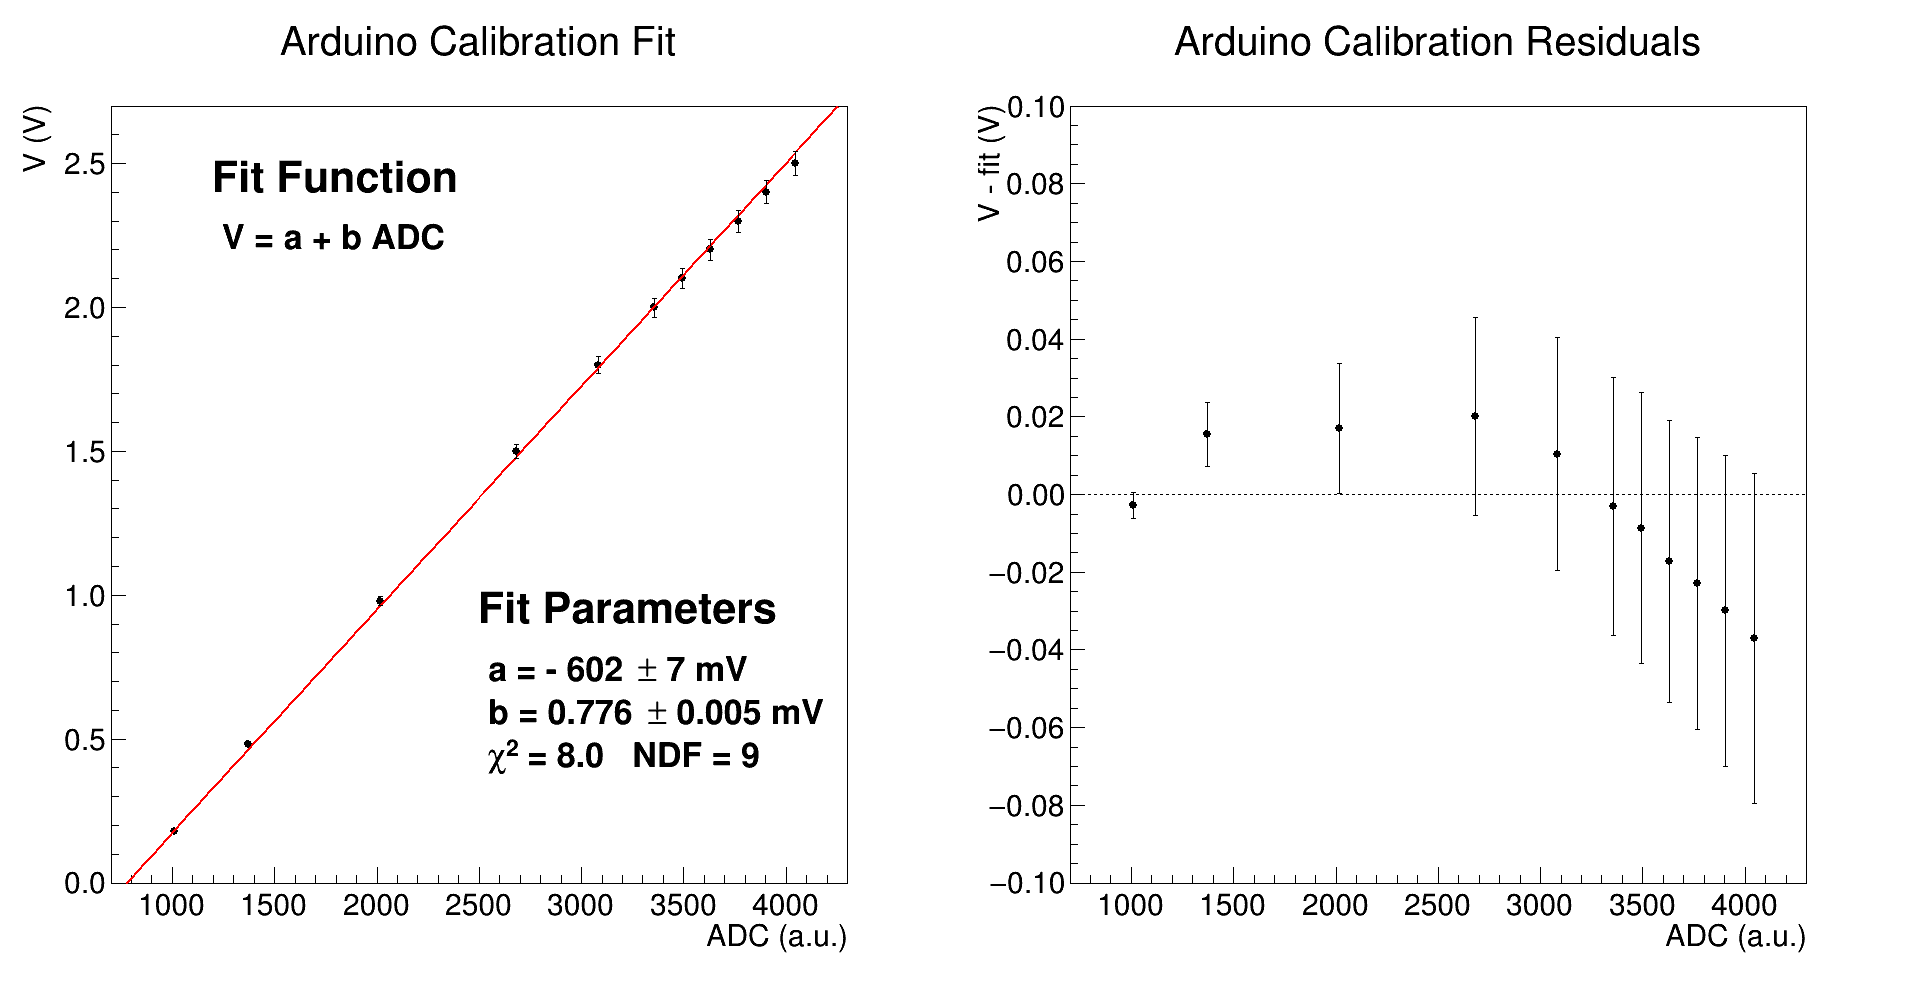
\includegraphics[width=15cm]{../Arduino/Plots/calib_function.png}
	\caption{Grafico di calibrazione in tensione e relativo grafico dei residui.}
	\label{i:ar_calib}
\end{figure}

\noindent 


%-------------------------------------------------------------------------------------------------------------------------------------------
%	CONCLUSIONI
%-------------------------------------------------------------------------------------------------------------------------------------------

\section{Conclusioni}

Ripercorrendo brevemente ciò che è emerso dall'analisi effettuata, si vuole cominciare osservando che la linearità
dell'amplificatore operazione è stata verificata dall'andamento dei residui in \autoref{i:opamp_pp} e dall'errore a
posteriori del campione di grandezze picco picco. Non è stato invece possibile fare riferimento ai valori di $\chi^2$ in
quanto la correlazione tra gli errori rende tali valori decisamente ridotti rispetto al numero di gradi di libertà.
Dalloo studio dell'amplificazione del circuito, rappresentato in \autoref{i:opamp_circuit}, è emersa poi una sistematica
di offset/shift verticale tra il campione di misure dei massimi e quello dei minimi. A causa di ciò, è stato necessario
considerare le grandezze picco picco per ricavare una stima che tenesse conto di entrambi i dataset e che fosse conforme
alle aspettative. La miglior stima dell'amplificazione del circuito risulta dunque essere $G=10.29 \pm 0.11$, ottenuta
come coefficiente angolare della retta interpolante il campione di grandezze picco picco. Spostando ora l'attenzione sul
circuito derivatore, dall'analisi in frequenza è emerso un comportamento più fedele ad un filtro passa banda piuttosto
che un passa alto (cioè l'aspettativa teorica) e si è ipotizzato che la causa fosse la presenza di una capacità
parassita in parallelo al circuito. La frequenza di taglio estrapolata attraverso la prima strategia si è ritrovata
essere scarsamente compatibile con le aspettative teoriche, e la causa di ciò potrebbe essere una campionatura troppo
rarefatta a basse frequenze che ha portato ad una stima non ottimale della retta a 20 dB/dec. L'interpolazione lineare
ristretta all'intorno della frequenza di taglio, nel quale la campionatura è sufficientemente fitta, invece restituisce
una stima $f_{\text{t}}=19.8 \pm 0.8\,\si{\kHz}$ in ottimo accordo con le aspettative. Si prende dunque quest'utlima
come miglior stima della frequenza di taglio. Per quanto riguarda la calibrazione della scheda Arduino Due, infine, si è
stimato un sampling rate di $955000$ acquisizioni al secondo e una funzione di calibrazione conforme alle aspettative,
ovvero con un coefficiente angolare $m=0.766\pm 0.013\,\text{mV/adc counts}$ e un offset $q=-0.59\pm0.02\,\si{\volt}$
per valori di tensione in ingresso sotto circa $2\,\si{\volt}$.


%----------------------------------------------------END OF FILE----------------------------------------------------------------------------
\end{document}